\documentclass[
	10pt,								% globale Schriftgröße
	parskip=half-,						% setzt Absatzabstand hoch
	paper=a4,							% Format
	english,ngerman,					% lädt Sprachpakete
	]{scrartcl}							% Dokumentenklasse

% //////////////////// Pakete laden ////////////////////
\usepackage{amsmath}			% MUSS vor fontspec geladen werden
\usepackage{mathtools}			% modifiziert amsmath
\usepackage{amssymb}			% mathematische symbole, für \ceckmarks
\usepackage{amsthm}				% für proof
\usepackage{mathrsfs}			% für \mathscr
\usepackage{latexsym}
\usepackage{marvosym}				% für Lightning

\usepackage{fontspec} 			% funktioniert nur mit den neueren Compilern z.B. XeLaTeX
\usepackage{microtype}			% für bessere Worttrennung
\usepackage[ngerman]{babel} 	% Spracheinstellung
\usepackage{lmodern}			% verändert verwendete Schriftart, damit sie weniger pixelig ist

\usepackage{verbatim}
\usepackage{listings}			% Für Quellcode

\usepackage{graphicx}
\usepackage{tabularx}			% für Tabellen mit gleicher Spaltenbreite und automatischen Umbrüchen
\usepackage{fullpage}
\usepackage{multirow}			% für multirow in tabulars
\usepackage{rotate}
\usepackage[cmyk,table]{xcolor} % um Farben zu benutzen, kann mehr als das Paket color
\usepackage[					% Verlinkungen
	colorlinks,					% farbige Schrift, statt farbiger Rahmen
	linktocpage,				% verlinkt im Abb.Verzeichnis Seitenzahl statt Bildunterschrift
	linkcolor=blue				% setzt Farbe der Links auf blau
	]{hyperref}					% nur für digitale Anwendungen, url = "http://www.example.com"
\usepackage{url}				% für Webadressen wie e-mail usw.: "\url{http://www.example.com}"

\usepackage{enumerate}			% für versch. Aufzählungezeichen wie z.B. a)
\usepackage{xspace}				% folgt ein Leerzeichen nach einem \Befehl, wird es nicht verschluckt.
\usepackage{cancel}				% für das Durchstreichen u.a. in Matheformeln mit \cancel
\usepackage{float}              % zum Forcieren der Position von figure-Umgebungen

% zum Zeichnen (u.a. von Graphen)
\usepackage{fp}
\usepackage{tikz}
\usetikzlibrary{tikzmark}			% für \tikzmark{toRemember}
\usetikzlibrary{positioning}	% verbesserte Positionierung der Knoten
\usetikzlibrary{automata}		% für Automaten (GTI)
\usetikzlibrary{arrows}
\usetikzlibrary{shapes}
\usetikzlibrary{decorations.pathmorphing}
\usetikzlibrary{decorations.pathreplacing}
\usetikzlibrary{decorations.shapes}
\usetikzlibrary{decorations.text}

% //////////////////// Syntaxhighlighting ////////////////////
\lstloadlanguages{Python, Haskell, [LaTeX]TeX, Java}
\lstset{
   basicstyle=\footnotesize\ttfamily,	% \scriptsize the size of the fonts that are used for the code
   backgroundcolor = \color{bgcolour},	% legt Farbe der Box fest
   breakatwhitespace=false,	% sets if automatic breaks should only happen at whitespace
   breaklines=true,			% sets automatic line breaking
   captionpos=t,				% sets the caption-position to bottom, t for top
   commentstyle=\color{codeblue}\ttfamily,% comment style
   frame=single,				% adds a frame around the code
   keepspaces=true,			% keeps spaces in text, useful for keeping indentation
							% of code (possibly needs columns=flexible)
   keywordstyle=\bfseries\ttfamily\color{codepurple},% keyword style
   numbers=left,				% where to put the line-numbers;
   							% possible values are (none, left, right)
   numberstyle=\tiny\color{codegreen},	% the style that is used for the line-numbers
   numbersep=5pt,			% how far the line-numbers are from the code
   stepnumber=1,				% nummeriert nur jede i-te Zeile
   showspaces=false,			% show spaces everywhere adding particular underscores;
							% it overrides 'showstringspaces'
   showstringspaces=false,	% underline spaces within strings only
   showtabs=false,			% show tabs within strings adding particular underscores
   flexiblecolumns=false,
   tabsize=1,				% the step between two line-numbers. If 1: each line will be numbered
   stringstyle=\color{orange}\ttfamily,	% string literal style
   numberblanklines=false,				% leere Zeilen werden nicht mitnummeriert
   xleftmargin=1.2em,					% Abstand zum linken Layoutrand
   xrightmargin=0.4em,					% Abstand zum rechten Layoutrand
   aboveskip=2ex, 
}

\lstdefinestyle{py}{
   language=Python,
}
\lstdefinestyle{hs}{
   language=Haskell,
}
\lstdefinestyle{tex}{
	language=[LaTeX]TeX,
	escapeinside={\%*}{*)},     % if you want to add LaTeX within your code
	texcsstyle=*\bfseries\color{blue},% hervorhebung der tex-Schlüsselwörter
	morekeywords={*,\$,\{,\},\[,\],lstinputlisting,includegraphics,
	rowcolor,columncolor,listoffigures,lstlistoflistings,
	subsection,subsubsection,textcolor,tableofcontents,colorbox,
	fcolorbox,definecolor,cellcolor,url,linktocpage,subtitle,
	subject,maketitle,usetikzlibrary,node,path,addbibresource,
	printbibliography},% if you want to add more keywords to the set
     numbers=none,
     numbersep=0pt,
     xleftmargin=0.4em,
}

\lstdefinestyle{java}{
	language=Java,
	extendedchars=true,		% lets you use non-ASCII characters;
   						% for 8-bits encodings only, does not work with UTF-8
}

\lstdefinelanguage[x64]{Assembler}     % add a "x64" dialect of Assembler
   [x86masm]{Assembler} % based on the "x86masm" dialect
   % with these extra keywords:
   {morekeywords={CDQE,CQO,CMPSQ,CMPXCHG16B,JRCXZ,LODSQ,MOVSXD, %
                  POPFQ,PUSHFQ,SCASQ,STOSQ,IRETQ,RDTSCP,SWAPGS, %
                  rax,rdx,rcx,rbx,rsi,rdi,rsp,rbp, %
                  r8,r8d,r8w,r8b,r9,r9d,r9w,r9b}
}					% for 8-bits encodings only, does not work with UTF-8

\lstdefinestyle{c}{
	language=c,
	extendedchars=true,		% for 8-bits encodings only, does not work with UTF-8
}

% //////////////////// eigene Kommandos ////////////////////
\newcommand\FU{Freie Universität Berlin\xspace}% benötigt package xspace
\newcommand\gdw{g.\,d.\,w.\xspace}
\newcommand\oBdA{o.\,B.\,d.\,A.\xspace}
\newcommand{\Eu}{\texteuro}
\newcommand\N{\mathbb{N}\xspace}
\newcommand\Q{\mathbb{Q}\xspace}
\newcommand\R{\mathbb{R}\xspace}
\newcommand\Z{\mathbb{Z}\xspace}
\newcommand\ohneNull{\ensuremath{\backslash\lbrace 0\rbrace}}% \{0}
\let\dhALT\dh	% Schreibt Befehl \dh in \dhALT um
\renewcommand\dh{d.\,h.\xspace}	%renew überschreibt command \dh
\newcommand\Bolt{\;\text{\LARGE\raisebox{-0.3em}{\Lightning}\normalsize}\xspace}% Blitz
\newcommand\zz{\ensuremath{\raisebox{+0.25ex}{Z}% zu zeigen
			\kern-0.4em\raisebox{-0.25ex}{Z}%
			\;\xspace}}
\newcommand{\from}{\ensuremath{\colon}}
\newcommand{\floor}[1]{\lfloor{#1}\rfloor}
\newcommand{\ceil}[1]{\lceil{#1}\rceil}
 \renewcommand{\L}{\ensuremath{\mathcal{L}}\xspace}
 \renewcommand{\P}{\ensuremath{\mathcal{P}}\xspace}
 \newcommand{\NL}{\ensuremath{\mathcal{N}\kern-0.2em\mathcal{L}}\xspace}
 \newcommand{\NP}{\ensuremath{\mathcal{NP}}\xspace}

% //////////////////// Mathefunktionen ////////////////////
\DeclareMathOperator{\Landau}{\mathcal{O}}
\DeclareMathOperator{\True}{True}
\DeclareMathOperator{\False}{False}

% //////////////////// eigene Theoreme ////////////////////
\newtheorem{theorem}{Satz}
\newtheorem{corollary}[theorem]{Folgerung}
\newtheorem{lemma}[theorem]{Lemma}
\newtheorem{observation}[theorem]{Beobachtung}
\newtheorem{definition}[theorem]{Definition}
\newtheorem{Literatur}[theorem]{Literatur}
% konfiguriert proof
\makeatletter
\newenvironment{Proof}[1][\proofname]{\par
  \pushQED{\qed}%
  \normalfont \topsep6\p@\@plus6\p@\relax
  \trivlist
  \item[\hskip\labelsep
%         \itshape
        \bfseries
    #1\@addpunct{.}]\ignorespaces
}{%
  \popQED\endtrivlist\@endpefalse
}
\makeatother

% //////////////////// eigene Farben ////////////////////
\let\definecolor=\xdefinecolor
\definecolor{FUgreen}{RGB}{153,204,0}
\definecolor{FUblue}{RGB}{0,51,102}

\definecolor{middlegray}{rgb}{0.5,0.5,0.5}
\definecolor{lightgray}{rgb}{0.8,0.8,0.8}
\definecolor{orange}{rgb}{0.8,0.3,0.3}
\definecolor{azur}{rgb}{0,0.7,1}
\definecolor{yac}{rgb}{0.6,0.6,0.1}
\definecolor{Pink}{rgb}{1,0,0.6}

\definecolor{bgcolour}{rgb}{0.97,0.97,0.97}
\definecolor{codegreen}{rgb}{0,0.6,0}
\definecolor{codegray}{rgb}{0.35,0.35,0.35}
\definecolor{codepurple}{rgb}{0.58,0,0.82}
\definecolor{codeblue}{rgb}{0.4,0.5,1}

% //////////////////// eigene Settings ////////////////////

\textheight = 230mm		% Höhe des Satzspiegels / Layouts
\footskip = 10ex			% Abstand zw. Fußzeile und Grundlinie letzter Textzeile
\parindent 0pt			% verhindert Einrückung der 1. Zeile eines Absatzes
\setkomafont{sectioning}{\rmfamily\bfseries}% setzt Ü-Schriften in Serifen, {disposition}
\usepackage{enumitem}
\usepackage{cite}
    \bibliographystyle{IEEEtran}
\usepackage{natbib}
\newcommand{\dozent}{Dr. Larissa Groth}
\newcommand{\veranstaltung}{IoT Network Security}
\newcommand{\semester}{SoSe23}
\newcommand{\studenten}{Zohreh Asadi, Aiman Al-Hazmi}
\begin{document}
% /////////////////////// BEGIN TITLEPAGE /////////////////////////
\begin{titlepage}
	\title{\veranstaltung}
	\subtitle{\Large Untersuchung der verschieden Schutzmechanismen in Smart Home Netzwerken, \semester}
	\author{\textbf{Autoren:} \studenten \\ \textbf{Dozentin:} \dozent}
	\date{\normalsize \today}
\end{titlepage}

\maketitle								% Erstellt das Titelblatt
\vspace*{-9cm}							% rückt Logo an den oberen Seitenrand
\makebox[\dimexpr\textwidth+1cm][r]{	%rechtsbündig und geht rechts 1cm über Layout hinaus
	
\includegraphics[width=0.4\textwidth]{src/fu_logo} % fügt FU-Logo ein
}
% /////////////////////// END TITLEPAGE /////////////////////////

\vspace{6cm}							% Abstand
\rule{\linewidth}{0.8pt}				% horizontale Linie
\tableofcontents
\newpage

\section{Einführung}

Die Bedenken hinsichtlich der Sicherheit und des Datenschutzes von IoT-Geräten nehmen zu, da Smart Homes immer beliebter und verbreiteter werden. Es gibt Hunderttausende Studien, die Sicherheitsrisiken und Gegenmaßnahmen in Smart-Home-Umgebungen identifizieren und bewerten. Dieser Artikel bietet einen Überblick über Sicherheits- und Datenschutzprobleme in Smart-Home-Netzwerken und konzentriert sich auf die Untersuchung verschiedener Schutzmechanismen. Die Rezension basiert auf einer Auswahl mehrerer Forschungsartikel und Bücher. Ziel des Beitrags ist es, einen detaillierten Überblick über die aktuellen Forschungsergebnisse zu geben und Empfehlungen und Ansichten zur Implementierung von Sicherheitsmechanismen in einer Smart-Home-Umgebung zu geben. 

Der Artikel beginnt mit einer Einführung in verschiedene Netzwerkarchitekturen und Kommunikationsprotokolle. Das Smart-Home-Netzwerk basiert auf einem grundlegenden Schichtenmodell bestehend aus der Sensor- und Aktorschicht, der Netzwerkschicht und der Anwendungsschicht. Die Kommunikation zwischen Geräten erfolgt über verschiedene Protokolle wie Wi-Fi, Bluetooth, Zigbee, Z-Wave, MQTT und CoAP. Anschließend geht er auf die Gefahren und Risiken ein, die mit Smart-Home-Netzwerken verbunden sind, und betont die Bedeutung der Sicherheit in einer IoT-Umgebung. Darüber hinaus werden verschiedene Cyberangriffe besprochen, die häufig in IoT-Anwendungen auftreten, wie zum Beispiel: B. Channel-Angriffe, selektive Umleitungsangriffe, Sybil-Angriffe und Denial-of-Service-Angriffe (DoS). 

Im weiteren Verlauf dieses Artikels werden die wichtigsten Sicherheitsmechanismen für Smart-Home-Netzwerke erörtert, wobei der Schwerpunkt auf der IoT-Authentifizierung und der Sicherheitsarchitektur liegt. Es werden Verschlüsselungs-, Authentifizierungs- und Zugriffskontrollmechanismen untersucht, darunter Technologien wie Advanced Encryption Standard (AES), Blowfish und RSA. Die Vorteile, Einschränkungen und Leistung dieser Verschlüsselungsalgorithmen werden diskutiert. Die Authentifizierung, insbesondere mittels CoAP, spielt eine wichtige Rolle bei der Gewährleistung der Sicherheit und Integrität der Kommunikation in einem Smart-Home-Netzwerk.

Insgesamt analysiert dieser Artikel Sicherheits- und Datenschutzprobleme in Smart-Home-Netzwerken und skizziert wichtige Sicherheitsmaßnahmen. Ziel ist es, das Verständnis für Cybersicherheit im Bereich IoT zu fördern und bei der Gestaltung einer sicheren Smart-Home-Umgebung zu helfen.


\section{Grundlagen von Smart Home Netzwerken}

\subsection{Architektur von Smart Home-Netzwerken}

In der Literatur wurden mehrere IoT-Architekturen vorgeschlagen. Die IoT-Architektur berücksichtigt wichtige Faktoren wie Dienstqualität (QoS), Datenschutz, Zuverlässigkeit, Integrität usw.\cite{8203943}. 
Die allgemeine IoT-Architektur besteht aus drei Hauptschichten: der  Wahrnehmungs- oder physischen Schicht, der Netzwerkschicht und der Anwendungsschicht. In diesem Abschnitt befassen wir uns mit der grundlegenden Architektur und Serviceorientierung des IoT.

\paragraph{Basic layered architecture}\

Die Verwendung dieser Architektur ist weit verbreitet, um Komponenten zu strukturieren und mit dem System zu interagieren. Diese  Architektur bietet einen modularen Ansatz, der Flexibilität, Skalierbarkeit und Interoperabilität bietet\cite{8203943}. Innerhalb dieser Architektur werden verschiedene Schichten verwendet, um spezifische Funktionen auszuführen.

\begin{enumerate}
    \item \textbf{Die Wahrnehmungsschicht} ist dafür verantwortlich, Daten von verschiedenen Sensoren und Geräten in der physischen Welt zu erfassen. Physische Ereignisse werden in digitale Daten umgewandelt, die verarbeitet und übertragen werden können. 

    \item \textbf{Die Netzwerkschicht} sorgt für die Kommunikation zwischen Geräten/Sensoren in der Wahrnehmungsschicht und den höheren Schichten der Architektur. Es umfasst Protokolle und Technologien wie Wi-Fi, Bluetooth, Zigbee, Mobilfunknetze und andere Konnektivitätsoptionen. Diese Schicht gewährleistet eine zuverlässige Datenübertragung und verwaltet die Kommunikation zwischen Geräten.

    \item \textbf{Die Anwendungsschicht} ist die oberste Schicht der Architektur und besteht aus verschiedenen IoT-Anwendungen und -Diensten. Diese Anwendungen nutzen verarbeitete Daten zur Durchführung spezifischer Funktionen wie Überwachung, Steuerung, Automatisierung, Analyse und Entscheidungsfindung. Beispiele für IoT-Anwendungen sind Smart-Home-Systeme, industrielle Überwachungssysteme sowie Gesundheits- und Umweltüberwachung.
\end{enumerate}

\begin{figure}[h]
  \centering
  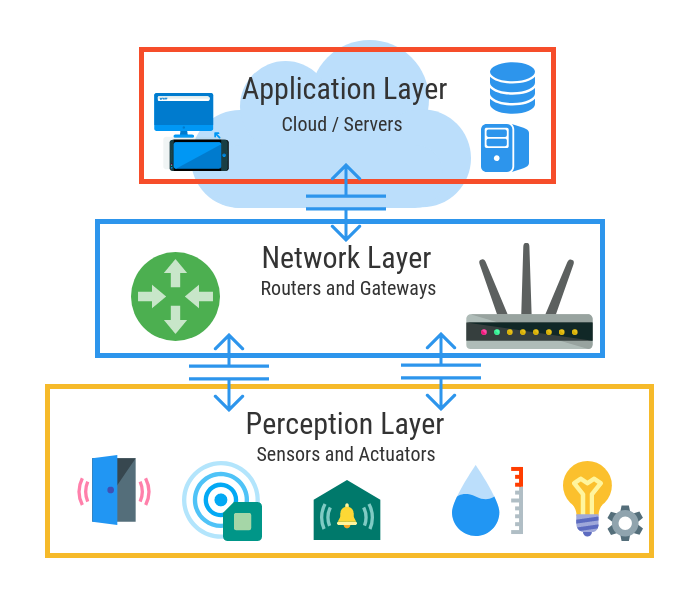
\includegraphics[scale=0.3]{resources/three-layer-iot-architecture.png}
  \caption{Basic layered architecture \href{https://www.netburner.com/learn/architectural-frameworks-in-the-iot-civilization/}{Quelle}.}
  \label{fig:Basic_architecture}
\end{figure}

\paragraph{Serviceorientierte Architektur}\

Die IoT-Architektur kann dienstorientiert sein. Ihre vier Schichten sind in Abbildung \ref{fig:Serviceorientierte} dargestellt. Die Erfassungsschicht (Sensing layer) integriert die Hardware. Die Netzwerkschicht unterstützt die Datenübertragung über das Netzwerk. Die Dienstschicht (Service layer) erstellt und verwaltet Dienste. Die Schnittstellenschicht (Interface layer) ermöglicht die Interaktion zwischen Benutzer und Anwendungen\cite{8203943}.


\begin{figure}[h]
  \centering
  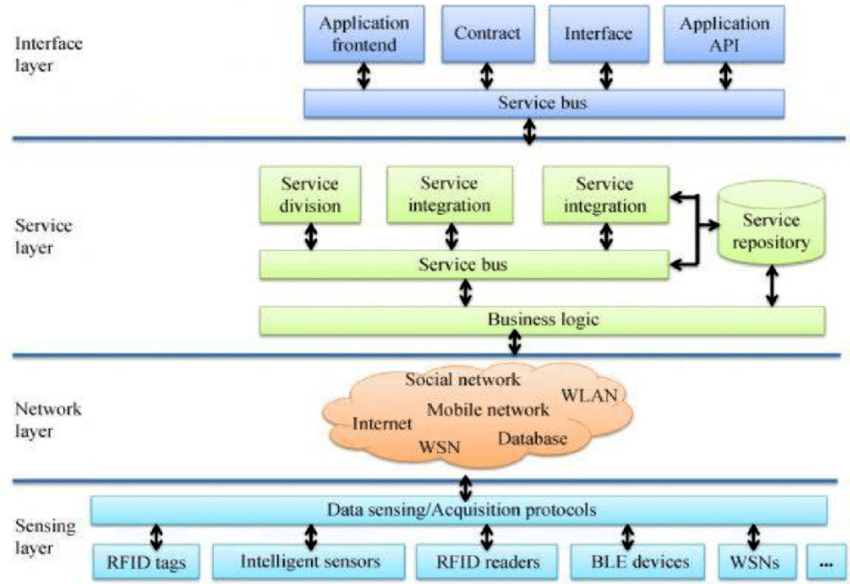
\includegraphics[scale=0.3]{resources/oT-service-oriented-architecture.png}
  \caption{Serviceorientierte Architektur \href{https://www.researchgate.net/figure/oT-service-oriented-architecture_fig1_348398089}{Quelle}}
  \label{fig:Serviceorientierte}
\end{figure}
\paragraph{Smart Homes Architektur}\

 Abbildung \ref{fig:Smart_Home} zeigt ein Beispiel einer Smart-Home Architektur.
Ein Smart Home besteht aus verschiedenen Geräten, die mit einem lokalen Netzwerk (LAN) verbunden sind. Diese Geräte kommunizieren untereinander über Kommunikationsprotokolle wie ZigBee, Bluetooth, Wi-Fi oder andere RF-Technologien. Die Smart-Home-Architektur besteht aus einem lokalen Netzwerk, das Geräte, Sensoren und Aktoren im Haus verbindet. Ein mit dem lokalen Netzwerk verbundener Server verwaltet Geräte, protokolliert, generiert Berichte und reagiert auf Benutzerbefehle. Der Server kann auch über APIs mit Cloud-Diensten interagieren und so zusätzliche Funktionalität und Skalierbarkeit bieten. Darüber hinaus sind Smart-Home-Geräte mit dem Internet verbunden, sodass Benutzer über die Anwendung aus der Ferne auf das System zugreifen und es steuern können\cite{djumanazarov2021overview}. 

\begin{figure}[h]
  \centering
  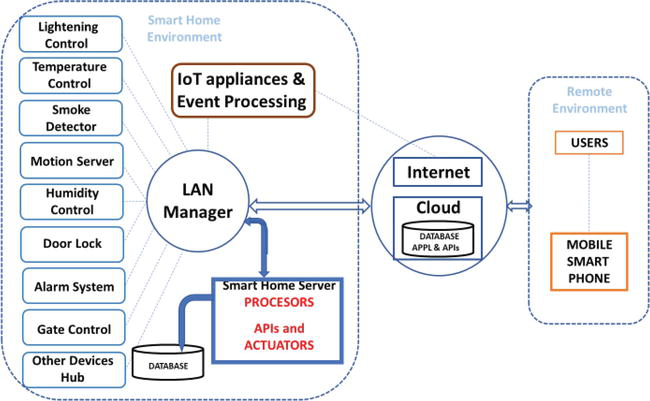
\includegraphics[scale=0.8]{resources/BuildinganIoT-basedarchitecturemodelforsmarthomes.png}
  \caption{Smart Homes Architektur \cite{djumanazarov2021overview}}
  \label{fig:Smart_Home}
\end{figure}

\subsection{Kommunikationsprotokolle in Smart Home Netzwerken}

Um in einem Smart Home effektiv kommunizieren zu können, müssen Geräte und Sensoren miteinander verbunden sein. Diese Verbindung basiert auf Kommunikationsprotokollen, die definieren, wie Daten zwischen diesen Geräten ausgetauscht werden. Diese Protokolle werden von verschiedenen Organisationen erstellt, um eine reibungslose und standardisierte Kommunikation in Smart-Home-Umgebungen sicherzustellen.

Die Wahl des Kommunikationsprotokolls für ein Smart-Home-System hängt von vielen Faktoren ab, unter anderem Verteilungsumgebung, Netzwerkgröße, Reichweite, Datenrate, Stromverbrauch und Netzwerkkonfiguration \cite{djumanazarov2021overview}\cite{khatoun2022cybersecurity}. Kommunikationsprotokolle können in drei Hauptgruppen unterteilt werden: kabelgebunden, drahtlos und hybrid. Kurze Erläuterungen zu häufig genannten Technologien für Smart-Home-Anwendungen:
\begin{enumerate}
    \item ZigBee: bietet eine robuste und skalierbare Lösung für die Verbindung und Steuerung verschiedener IoT-Geräte wie Sensoren, Aktoren, Beleuchtung, Thermostate und Smart-Home-Geräte\cite{8203943}\cite{khatoun2022cybersecurity}.  Der ZigBee-Protokollstapel besteht aus vier Schichten: der Anwendungsschicht, der Netzwerk- und Sicherheitsschicht, der MAC-Schicht und der PHY-Schicht\cite{8203943}. 
    \item Bluetooth: ist ein drahtloses Medium mit kurzer Reichweite, das zum Datenaustausch zwischen zwei Geräten über eine kurze Distanz verwendet wird\cite{khatoun2022cybersecurity}. 

    \item WiFi: ermöglicht drahtlose Kommunikation und ermöglicht den Zugriff auf das Internet in Form eines Funksignals \cite{8203943}.

      \item 6LoWPAN (IPv6 over Low-Power Wireless Personal Area Networks): ist ein Netzwerkprotokoll, das IPv6-Kommunikation über drahtlose Netze mit geringem Stromverbrauch ermöglicht\cite{khatoun2022cybersecurity}. Es bietet eine Lösung für die Anbindung ressourcenbeschränkter IoT-Geräte an IPv6-Netzwerke, indem es die Header-Größen reduziert und den Adressierungsraum optimiert, so dass diese Geräte auf IP-basierte Dienste und Kommunikation zugreifen können\cite{khatoun2022cybersecurity}.
      
          \item TLS (Transport Layer Security): ist ein Protokoll, das eine sichere und zuverlässige Kommunikation zwischen Anwendungen über das Internet gewährleistet\cite{khatoun2022cybersecurity}\cite{info7030044}. TLS befindet sich zwischen der Anwendungsschicht (z. B. HTTP) und der Transportschicht (z. B. TCP) und ermöglicht die Server-Authentifizierung, eine sichere und zuverlässige Verbindung sowie die Client-Authentifizierung mit Hilfe der Public-Key-Kryptografie\cite{khatoun2022cybersecurity}. TLS ist auch die verbesserte Version von SSL, mit der gleichen Architektur und den gleichen Protokollen \cite{khatoun2022cybersecurity}. Die einzigen Unterschiede sind einige Änderungen bei den Sicherheitsparametern und der Berechnung von MAC, Schlüsselblock und digitaler Signatur. Außerdem werden einige neue Warnmeldungen und Pseudozufallsfunktionen eingeführt, um die Sicherheit im Vergleich zu SSL zu erhöhen\cite{satapathy2016comprehensive}\cite{khatoun2022cybersecurity}. Sowohl SSL als auch TLS unterstützen eine breite Palette von Verschlüsselungsalgorithmen. Die Wahl des Verschlüsselungsalgorithmus erfolgt während des Handshake-Prozesses auf der Grundlage der von Client und Server unterstützten Algorithmen.
    \item Message Queuing Telemetry Transport (MQTT): funktioniert mit dem Übertragungs-/Internet -Steuerungsprotokoll (TCP/IP), der eine Verbesserung ermöglicht, die mit Verlusten behandelt wird. Es handelt sich um ein Client-Server-Nachrichtenprotokoll, das Nachrichten mit minimiertem Transport-Overhead übermittelt \cite{8203943}. Es gibt drei Dienstgüteklassen (QoS) für das MQTT-Protokoll, nämlich:
 'at most once', das sicherstellt, dass Nachrichten je nach Verfügbarkeit der Betriebsumgebung zugestellt werden, 
'at least once', das die Ankunft der Nachricht sicherstellt und
 'genau einmal', das die Ankunft der Nachricht genau einmal sicherstellt\cite{8203943}\cite{khatoun2022cybersecurity}. 
MQTT verfügt über einen erstaunlichen Mechanismus zur Benachrichtigung über eine anormale Unterbrechung der Verbindung.



    \item Constrained Application Protocol (CoAP):  ist ein Protokoll der Anwendungsschicht, das speziell für eingeschränkte Geräte entwickelt wurde\cite{8203943}\cite{khatoun2022cybersecurity}. Es ermöglicht einen effizienten Datenaustausch mithilfe eines REST-Modells (Representative State Transition) unter Verwendung von Methoden wie GET, PUT, POST und DELETE. Die Kommunikation zwischen zwei Knoten wird nicht gesichert\cite{oliver2022lightweight}. Für eine sichere Kommunikation verwendet CoAP DTLS (Data Transport Layer Security), da die Implementierung von TLS (Transport Layer Security) bei begrenzten Geräten schwierig ist. UDP-basiertes DTLS eignet sich für beengte Umgebungen\cite{khatoun2022cybersecurity}.
Eingeschränkte Geräte verfügen oft über begrenzte Ressourcen, z.B 8-Bit-Mikrocontroller mit minimalem RAM und ROM. Darüber hinaus weisen begrenzte Netze oft eine hohe Paketfehlerrate auf. CoAP geht auf diese Einschränkungen ein, indem es Webanforderungen wie Multicasting erfüllt, den Overhead minimiert und Einfachheit bietet \cite{8203943}.


    \item WebSocket: bietet eine zweiseitige Kommunikation mit dem Server, die aus einem Handshake und einem anschließenden Message Framing besteht. Die Interaktion zwischen Browser und Webserver nimmt zu, da sie die Übertragung von Echtzeitdaten vom und zum Server erleichtert. Websocket bietet Vollduplex-Kommunikation.\cite{8203943}

\end{enumerate}
\subsection{Bedrohungen und Risiken für Smart Home-Netzwerke}

Die Gewährleistung der Sicherheit in IoT-Umgebungen ist zu einer großen Herausforderung und einem wichtigen Barriers für den Fortschritt der Smart-Home-Automatisierung geworden \cite{10.1145/1978942.1979249} .Diese Anerkennung unterstreicht ihre Komplexität und Bedeutung.
Je mehr Smart-Home- und IoT-Geräte entwickelt werden, desto schneller nehmen die mit deren Nutzung verbundenen Gefahren, Bedrohungen und Risiken zu. Hier überprüfen wir zwei verschiedene Studien. In \cite{8344666} verwenden sie eine Methode namens 'Taxonomy'; welche ist ein System zur Inhaltsverwaltung, das Informationen basierend auf als Metadaten gespeicherten Begriffen gruppiert, und durch die Analyse der vorhandenen Literatur zu Smart Homes wurde eine Reihe von Bedrohungen identifiziert, die speziell für den Bereich Smart Home gelten. Basierend auf dieser Untersuchung gibt es 28 verschiedene Arten von Threads, die in drei verschiedene Gruppen eingeteilt werden können, nämlich: Unintentional, Malfunction und Intentional Threads.

\subsubsection{Threads}

\textbf{Intentional Threads:} 
Vorsätzlicher Missbrauch birgt Sicherheitsrisiken für Smart-Home-Geräte durch Aktivitäten wie Identitätsbetrug, Denial-of-Service-Angriffe und Datenmanipulation. Diese Aktionen können verschiedene zerstörerische Auswirkungen haben, darunter unbefugte Änderungen an Richtlinien, Identitätsdiebstahl und die Ausnutzung von Smart-Home-Diensten.

\textbf{Malfunction Threads:} 
Ausfälle im Internet oder Hardware- oder Softwarefehler, die zu internen Störungen und Kommunikationskanalausfällen führen können, sind die häufigsten Beispiele für Störungsthreads und -risiken in Smart Homes. Ein weiteres Beispiel sind Schäden durch Geräte oder Sensoren Dritter, die zu Fehlfunktionen des Geräts führen, die einen Austausch und einen vorübergehenden Funktionsverlust erfordern. Darüber hinaus beeinträchtigt die Installation nicht vertrauenswürdiger Hardware von Drittanbietern die Gerätesicherheit.

\textbf{Unintentional Threads:} 
Zu den unbeabsichtigten Threads gehören der Erhalt von Informationen aus unbekannten Quellen oder zufällige Änderungen von Daten oder Richtlinien. Dies geschieht normalerweise, wenn die Sicherheitsrichtlinien des Geräts nicht richtig eingestellt sind oder die Installation schwach ist. Die Nachteile dieser Art von Threads können Fehlfunktionen und Funktionsverluste sein.

In einer weiteren Studie \cite{JACOBSSON2016719} wurde die Risikoexposition von SHAS (sichere Hashing-Algorithmen) mithilfe der Methode der Information Security Risk Analysis (ISRA) untersucht.
Laut dieser Studie ist die Risikoanalyse im Internet der Dinge das größte Sperre für die Weiterentwicklung dieser Technologie. Der Zweck der Studie dieser Gruppe besteht darin, die Risiken zu verstehen, die mit der Nutzung und dem Missbrauch von Informationen in Smart Homes und Gebäuden verbunden sind, was für die Gewährleistung der Sicherheit in IoT-Umgebungen sehr wichtig ist. Von den 32 von dieser Gruppe untersuchten Risiken wurden 9 Fälle als geringes Risiko und 4 Fälle als hohes Risiko eingestuft. Hochrisikofaktoren hängen entweder mit dem menschlichen Faktor oder mit den Softwarekomponenten des Systems zusammen. 
Wenn wir die Risiken in Bezug auf Software oder Hardware kategorisieren, hängt das wahrscheinlichste Risiko in der Liste der softwarebezogenen Risiken mit einer unzureichenden Reaktionsfähigkeit des internen Gateways zusammen. Beispielsweise werden Systemereignisse nicht aufgezeichnet, was die Situation erschweren kann, später nachvollziehen. Der höchste Risikowert steht im Zusammenhang mit unbefugten Änderungen an Systemfunktionen in mobilen Anwendungen. Beispielsweise können Endbenutzer ohne entsprechende Anmeldeinformationen auf Systemressourcen zugreifen.
In der Kategorie der hardwarebezogenen Risiken sind die schwerwiegendsten Folgen hingegen mit unbefugten Änderungen bzw. Manipulationen an physischen Sensoren oder internen Gateways verbunden. Die höchsten Risikowerte beziehen sich auf unbefugte Änderungen/Manipulationen des internen Ports, beispielsweise das Zurücksetzen des Systems zur Wiederherstellung des Standardkennworts.

\subsubsection{Cyber-attacks}

Nachdem die verschiedenen Kategorien von Bedrohungen untersucht wurden und Einblicke in die Risiken und die Risikoexposition von Secure Hashing Algorithms (SHAS) gewonnen wurden, wird es Zeit, in die Welt der Cyberangriffe einzutauchen, die potenzielle Bedrohungen für Smart Homes und Gebäude im Internet der Dinge (IoT) darstellen. Das Verständnis und der Schutz vor diesen Angriffen sind entscheidende Aspekte, um eine robuste Sicherheit in IoT-Geräten zu gewährleisten.

Einige der häufig vorkommenden Cyberangriffe auf IoT-Anwendungen:

\boldsymbol{Sinkhole-Angriff:}
Ein Sinkhole-Angriff ist eine Art Angriff auf Netzwerkebene, der auftritt, wenn Daten während der Übertragung weitergeleitet werden. Bei diesem Angriff werden alle durch das Netzwerk fließenden Daten an einen kompromittierten Knoten im Netzwerk umgeleitet \cite{7001385} .Dieser Angriff reduziert den Datenverkehr und täuscht den Absender und das Netzwerk vor, dass das Paket sein eigentliches Ziel erreicht hat. Bei diesem Angriff handelt es sich um einen aktiven Angriff, der durch die Generierung von Datenverkehr und die Unterbrechung von Routing-Pfaden zu einem Denial-of-Service-Angriff (DoS) führen kann \cite{stephen2017intrusion} .

\boldsymbol{Selektiver Weiterleitungsangriff:}
Bei diesem Angriff werden ein oder mehrere Knoten im Netzwerk von den Hackers einnimmt. Wenn einer der Knoten ein Paket als selektiven Weiterleitungsangriff verwirft, helfen andere dabei, den Angriff zu verschleiern. Dies führt zu Paketverlusten aufgrund von Interferenzen und ist schwer zu erkennen. Dieser Angriff kann dazu führen, dass unvollständige Informationen übertragen werden und deren Integrität beeinträchtigt wird. In manchen Anwendungen können unvollständige Informationen sogar gefährlicher sein als keine Informationen \cite{s16010118} .

\boldsymbol{Sybil-Angriff:}
Es ist ein weiterer Angriff auf Netzwerkebene, bei dem Angreifer Knoten manipulieren und mehrere Identitäten für einen einzelnen Knoten erstellen. Diese Art von Angriff gefährdet das gesamte System und kann zu Redundanz und falschen Informationen führen \cite{pawar2016sybil} .In IoT-Netzwerken werden Sensoren in Objekte eingebettet, die Sensorik und Kommunikation integrieren. Bei diesem Angriff wird eine gefälschte Identität generiert. Diese gefälschten Identitäten können falsche Berichte generieren, den Spam-Verkehr erhöhen und die Privatsphäre durch Malware und Phishing gefährden \cite{alqassem2014privacy} .

\boldsymbol{DoS-Angriff:}
Ein DoS-Angriff kann sowohl auf der Netzwerkebene als auch auf der Anwendungsebene erfolgen. Bei diesem Angriff überschwemmt der Angreifer das Netzwerk mit nutzlosem Datenverkehr (mehrere gleichzeitige Angriffe auf denselben Server) mit dem Ziel, Netzwerkressourcen zu belasten. Dieser Angriff macht das Netzwerk für legitime Benutzer unzugänglich \cite{kozlov2012security} .Auf der Anwendungsebene ist der Angriff sogar noch ausgefeilter, da er die Netzwerkverteidigung umgeht und vertrauliche Informationen unter der Kontrolle des Angreifers stiehlt. Dieser Angriff kann auch dazu führen, dass das gesamte Netzwerk heruntergefahren wird und nicht mehr verfügbar ist\cite{pawar2016sybil}.

\subsection{Wichtige Schutzmechanismen zur Sicherung von Smart Home-Netzwerken} 
Um die Sicherheit eines mit dem Internet verbundenen Smart-Home-Systems zu gewährleisten, ist es wichtig, sieben Schlüsselkonzepte der Computersicherheit zu berücksichtigen und anzugehen \cite{khatoun2022cybersecurity}\cite{smys2020hybrid}:
 \begin{enumerate}
     \item \textbf{Authentifizierung:} Der Prozess der Überprüfung der Identität einer Person, eines Systems oder eines Objekts, um diese Identität sicherzustellen.
\item \textbf{Autorisierung:} Der Prozess der Bestimmung, welche Berechtigungen, Zugriffe oder Berechtigungen einer authentifizierten Person, einem authentifizierten System oder einer authentifizierten Entität gewährt werden. Es definiert, auf welche Ressourcen oder Informationen sie Zugriff haben und welche Maßnahmen sie ergreifen können.
\item \textbf{Vertraulichkeit:} Die Sicherstellung, dass Informationen nur von autorisierten Personen eingesehen oder genutzt werden können.

\item \textbf{Integrität} der Daten/Nachrichten: Die Sicherstellung, dass Daten oder Nachrichten während der Speicherung, Übertragung oder Verarbeitung nicht unabsichtlich verändert oder manipuliert wurden.
\item \textbf{Accountability:} Die Fähigkeit, Handlungen und Aktivitäten einer Person, eines Systems oder einer Entität nachzuverfolgen und für diese verantwortlich zu sein. Es ermöglicht die Identifizierung von Personen, die für bestimmte Aktionen verantwortlich sind.
\item \textbf{Verfügbarkeit:} Informationen, Systeme oder Ressourcen sollten jederzeit und für autorisierte Benutzer zugänglich sein. Es beinhaltet die Gewährleistung, dass Dienste oder Ressourcen nicht durch Ausfälle, Angriffe oder andere Störungen beeinträchtigt werden.
\item \textbf{Nicht-Abstreitbarkeit:} Die Fähigkeit, die Authentizität und Integrität einer Kommunikation oder Transaktion nachzuweisen und sicherzustellen, dass die beteiligten Parteien später nicht leugnen können, dass sie an der Kommunikation oder Transaktion beteiligt waren. 
 \end{enumerate}


Verschiedene Arten von Angriffen können die Sicherheit physischer Objekte oder die Sicherheit kognitiver Daten gefährden. Zum Schutz der Wahrnehmungsebene (perception layer)  sollten verschiedene Sicherheitsmethoden eingesetzt werden, darunter B. Authentifizierungs- und Zugriffskontrollverfahren, Datenintegritäts- und Sicherheitsverfahren sowie Schlüsselverwaltungssysteme\cite{saadeh2016authentication}.

 Die Netzwerkschicht leidet unter mehreren Sicherheitsproblemen und verschiedenen Arten von Angriffen, wie z. Man-in-the-Middle-Angriffe, Listening-Angriffe, DoS-Angriffe, Replay-Angriffe, Authentifizierungsprobleme, Datenintegrität und Datenschutz, Routing-Sicherheitsprobleme und Datenschutzrisiken\cite{saadeh2016authentication}\cite{khatoun2022cybersecurity}.


\paragraph{IoT-Sicherheitsarchitekturen}
\

IoT-Sicherheitsarchitekturen
Die IoT-Sicherheitsforschung hat zur Entwicklung verschiedener Architekturen geführt, darunter Cloud Computing (CoT), Fog Computing, Edge Computing und Gateway-Architektur. Für die Kommunikation mit IoT-Geräten werden üblicherweise Middleware-Systeme verwendet\cite{khatoun2022cybersecurity}. Diese Architekturen zielen darauf ab, die Sicherheit zu verbessern und Lösungen für komplexe Verarbeitung, echtzeitnahe Reaktionen und zentralisierte Koordinationbereitzustellen. Die Gateway-Architektur bietet Proxy-Unterstützung auch dann, wenn keine Verbindung besteht\cite{khatoun2022cybersecurity}.

Hier ist eine verkürzte Liste einiger sicherer IoT-Architekturen \cite{khatoun2022cybersecurity}:

 \begin{enumerate}
 \item FIWARE (2011): ist eine IoT-Middleware mit einem Framework, das eine Vielzahl von Plugins unterstützt. Die Sicherheit wird durch Plugins für die Identitätsverwaltung, die Autorisierungspolitik und die Punkte zur Durchsetzung von Richtlinien implementiert.
    \item IoT Cloud on CoAP(2014): Cloudbasierte IoT-Architektur basierend auf CoAP und unter Verwendung von DTLS für die Sicherheit.

    \item IAGW(2016): Integrierte Gateway-Architektur mit Standardschnittstellen für Smart-Home-Umgebungen, inklusive Sicherheitsmodul zur Authentifizierung, Autorisierung und Verschlüsselung.
    \item Smart-Home-Automatisierung mit WSN(2019): verwendet den Triangle Based Security Algorithm (TBSA), um eine energieeffiziente Datenverschlüsselung zu gewährleisten und so ein sicheres IoT-basiertes Smart-Home-Automatisierungssystem zu schaffen.
    
    \item SH-BlockCC (2019): Dies ist eine sichere IoT-Smart-Home-Architektur, die auf Blockchain- und Cloud-Computing-Technologie basiert. Blockchain ist eine dezentrale und verteilte Datenbank, die Transparenz, Integrität und Sicherheit bieten kann\cite{singh2019sh}\cite{dorri2017blockchain}. Das Modell verwendet die MCA-Methode (Multivariate Correlation Analysis), um den Netzwerkverkehr zu analysieren und die Korrelation zwischen Verkehrsmerkmalen zu bestimmen.
 \end{enumerate}
Die folgende Tabelle \ref{fig:vergleich} fasst die Sicherheitsarchitekturen und die Sicherheitsziele zusammen, die sie jeweils zu schützen versprechen \cite{khatoun2022cybersecurity}.

\begin{figure}[h]
  \centering
  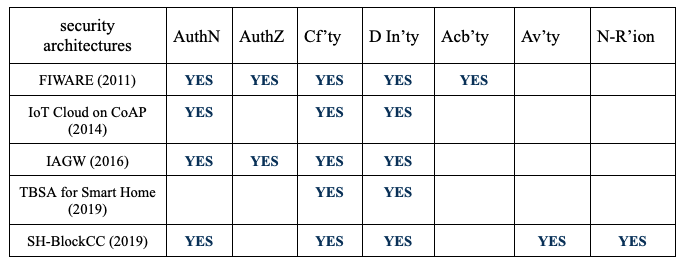
\includegraphics[scale=0.48]{resources/vergleich.png}
  \caption{Matrix of security architectures and security goals (Authentication (AuthN), Authorization (AuthZ), Confidentiality (Cf’ty), Data Integrity (D In’ty), Accountability (Acb’ty), Availability (Av’ty), Non-Repudiation (N-R’ion))}
  \label{fig:vergleich}
\end{figure}\


\paragraph{SH-BlockCC}\

Die Blockchain-Technologie kann als wichtiger Sicherheitsmechanismus zum Schutz von Smart-Home-Netzwerken eingesetzt werden. Unter Blockchain versteht man eine dezentrale Struktur, in der es keine einzige Autorität gibt, die Transaktionen genehmigt. Die Transaktionen beziehen sich in diesem Kontext auf die Interaktion und Kommunikation zwischen lokalen Smart-Home Geräten und den Overlay-Netzwerken. Abhängig von der Funktionalität können unterschiedliche Arten von Transaktionen zwischen Geräten und Overlay-Netzwerken stattfinden, beispielsweise Zugriffstransaktionen, Speichertransaktionen und Überwachungstransaktionen. Diese Transaktionen werden auf der lokalen Blockchain verwaltet und gespeichert. Um das Vertrauen in die Blockchain sicherzustellen, müssen die Knoten im Netzwerk einen Konsens zur Annahme von Transaktionen erzielen\cite{singh2019sh}, \cite{dorri2017blockchain}, \cite{khatoun2022cybersecurity}. 

Nach dem Hinzufügen eines neuen Geräts zum Smart-Home Netzwerk führt das Netzwerk eine Genesis-Transaktion durch, um die Anwesenheit des Geräts zu registrieren und zu überprüfen. Diese Transaktion enthält wichtige Geräteinformationen wie z.B Seine ID und einzigartige Merkmale. Um eine sichere Kommunikation im Smart Home zu gewährleisten, wird bei der Genesis-Transaktion ein gemeinsamer Schlüssel mithilfe eines Verschlüsselungsalgorithmus wie Diffie-Hellman generiert. Mit diesem Schlüssel kann das neue Gerät sicher mit dem Netzwerk interagieren und sich authentifizieren. Miner, die für die Netzwerkwartung und -validierung verantwortlich sind, weisen Geräten basierend auf den von Smart-Home-Besitzern festgelegten Regeln gemeinsame Schlüssel zu. Auf diese Weise steuern Benutzer Netzwerktransaktionen und Geräte können sicher miteinander kommunizieren\cite{singh2019sh}\cite{dorri2017blockchain}.



\paragraph{Intrusion-Detection-Systeme (IDS)}
\

Intrusion-Detection-Systeme (IDS) sind für die Netzwerk- und Datensicherheit von entscheidender Bedeutung. Sie erkennen und verhindern unbefugten Zugriff, und ein zentralisierter IDS-Ansatz kann den Einsatz bei begrenzter Stromversorgung vereinfachen. IDS arbeitet in drei Phasen: Überwachung, Analyse und Erkennung. Es verwendet Sensoren, um das Netzwerk oder den Host zu beobachten, Merkmale zu extrahieren und Muster während der Analyse zu identifizieren, und konzentriert sich bei der Erkennung auf die Identifizierung von Anomalien oder Eindringlingen. IDS entwickeln sich im Laufe der Zeit weiter und für verschiedene Systeme wurden unterschiedliche Methoden und Techniken vorgeschlagen. Durch die effiziente Verwaltung von Informationen, Diensten und Netzwerkverkehr verbessert IDS die Netzwerksicherheit, den Datenschutz und die Integrität\cite{smys2020hybrid}\cite{elrawy2018intrusion}.

\paragraph{Verschlüsselung, Authentifizierung und Zugriffskontrolle}
\

Bei der Authentifizierung wird die Identität einer Person oder eines Geräts überprüft, um sicherzustellen, dass es sich um das handelt, was es vorgibt zu sein. Dieser Sicherheitsmechanismus dient dazu, unbefugten Zugriff auf das System, Daten oder Ressourcen zu verhindern. Dies werden wir genauer  später in diesem Artikel betrachten.

\section{Verschlüsselung, Authentifizierung und Zugriffskontrolle in Smart Home-Netzwerken}
\subsection{Verschlüsselungstechnologien}

Verschlüsselungstechnologien spielen eine entscheidende Rolle bei der Sicherung von sensiblen Informationen und der Gewährleistung der Privatsphäre. 
Für die Kryptographie wurden verschiedene Ziele aufgeführt, nämlich: Vertraulichkeit, Authentifizierung, Integrität, Bestreitbarkeit und Zugangskontrolle. 

Verschlüsselungsalgorithmen können in zwei große Kategorien eingeteilt werden: Verschlüsselung mit symmetrischem Schlüssel (z. B. AES, Blowfish) und Verschlüsselung mit asymmetrischem Schlüssel (z. B. RSA).\cite{thambiraja2012survey} .
Symmetrische Verschlüsselung, auch als Geheimschlüsselverschlüsselung bekannt, ist eine grundlegende kryptografische Technik zur Sicherung sensibler Informationen. Dabei wird ein einziger geheimer Schlüssel für sowohl den Verschlüsselungs- als auch den Entschlüsselungsprozess verwendet.
Auf der anderen Seite verwendet die asymmetrische Verschlüsselung, auch bekannt als Public-Key-Verschlüsselung, ein Schlüsselpaar: einen öffentlichen Schlüssel zum Verschlüsseln von Daten und einen privaten Schlüssel zum Entschlüsseln \cite{khatoun2022cybersecurity}.

Im Folgenden besprechen wir zwei symmetrische Verschlüsselungsalgorithmen, nämlich AES (Advanced Encryption Standard) und Blowfish, sowie einen asymmetrischen Verschlüsselungsalgorithmus RSA.


\subsubsection{AES:}

AES (Advanced Encryption Standard) ist ein symmetrischer Verschlüsselungsalgorithmus, der mit Datenblöcken arbeitet. Es verwendet schlüsselbasierte Ersetzungs- und Permutationsoperationen, um Vertraulichkeit und Datenintegrität sicherzustellen. AES umfasst eine Schlüsselerweiterung zur Generierung von Rundenschlüsseln und durchläuft mehrere Runden von Substitutions-, Shift-, Shuffle- und XOR-Operationen. Der Verschlüsselungsprozess wandelt Klartext in Chiffretext um, während die Entschlüsselung die Schritte umkehrt, um den ursprünglichen Klartext abzurufen.\cite{abdullah2017advanced}
The AES design is based on a substitution-permutation network 
(SPN) and does not use the Data Encryption Standard (DES) Feistel network\cite{raghav2016securing}.
Einerseits weist AES eine schlechte Leistung auf, da es mehr Rechenleistung benötigt und bei großen Datenblöcken mehr Ressourcen verbraucht. Andererseits ist es für kleine Pakete sogar besser als viele Algorithmen, einschließlich RC4, außerdem hat AES keine Wurmlöcher.\cite{abdullah2017advanced}
Wie in\ref{fig:vergleich5} erwähnt, verfügt AES über eine schnelle Ver- und Entschlüsselung und verfügt über eine Schlüsselgröße von 128, 192 und 256 Bit. Seine Geschwindigkeit hängt vom Schlüssel ab, es ist aber sicher und funktioniert besser als viele Algorithmen, einschließlich DES und Triple-DES, und es ist sowohl in der Hardware als auch in der Software schnell\cite{devi2015review}, \cite{abdullah2017advanced}.


\subsubsection{BLOWFISH:}

Die Leistung des BLOWFISH-Algorithmus für unterschiedliche Paketgrößen mit und ohne Datentransformation ist besser als bei anderen Algorithmen und hat keine Wurmlöcher, aber er ist zeitaufwändig und verbraucht letztendlich mehr Strom\cite{thambiraja2012survey}.
Die Ver- und Entschlüsselung im BLOWFISH-Algorithmus erfolgt schnell und die Schlüsselgröße liegt zwischen 32 und 448 Bit. Die Geschwindigkeit dieses Algorithmus hängt nicht vom Schlüssel ab. Es wird angenommen, dass es gesichert ist, aber es gibt weniger Versuche zur Kryptoanalyse. Dieser Algorithmus wurde nur für Software entwickelt\cite{devi2015review}, \cite{thambiraja2012survey}.

Um die Daten mit BLOWFISH-Algorithmus zu verschlüsseln, sind folgende Schritte erforderlich:

1. Speichern Sie die Schlüssel in einem Array; k1,k2,...kn und 1<=n<=14
und die Länge jedes Blocks beträgt 32 Bit.\begin{align*}
32*14=448 \end{align*}
2. Initialisieren Sie das Array mit der Nummer p; 1<=p<=18, die Länge jedes Wortes beträgt 32 Bit.

3. Substitutions-Boxen initialisieren, jede darf maximal 255 Bit lang sein\begin{align*}
    2^8 -1 = 255 \end{align*}.
4. Initialisieren Sie jedes P-Array und S-Bixes mit Hexadezimalzahlen

5. Ausführen von XOR-Operationen zwischen k- und p-Arrays:\begin{align*} p1 = p1 XOR k1, ..., p14 = p14 XOR k14 \end{align*} \begin{align*} p15 = p15 XOR k1 , ... , p18 = p18 XOR k4.\end{align*}
6. Nehmen Sie 64-Bit-Klartexte und initialisieren Sie sie mit Null (000000).

Subkey wird generiert.
Create figure for this algo

\subsubsection{RSA:}

RSA ist ein Asymmetric-Algorithm, dass auf Verschlüsselung mit öffentlichen Schlüsseln und digitalen Signaturen basiert hat. Bei RSA sind Verschlüsselungsschlüssel öffentlich verfügbar, während Entschlüsselungsschlüssel privat bleiben. Dadurch kann jeder eine Nachricht mit dem öffentlichen Verschlüsselungsschlüssel des Empfängers verschlüsseln, aber nur der beabsichtigte Empfänger kann sie mit dem entsprechenden privaten Entschlüsselungsschlüssel entschlüsseln. Seine Sicherheit basiert auf der Schwierigkeit von folgenden Zahlen:

„p“ und „q“: Dabei handelt es sich um unterschiedliche Primzahlen, die zufällig ausgewählt werden. Die Sicherheit von RSA beruht auf der Schwierigkeit, das Produkt dieser beiden Primzahlen zu faktorisieren. Diese Primzahlen werden geheim gehalten und zur Generierung des privaten Schlüssels verwendet.

„n“: Dies ist das Produkt der beiden Primzahlen „p“ und „q“ (n = p*q). Es ist Teil sowohl des öffentlichen als auch des privaten Schlüssels. Der Wert von „n“ ist öffentlich und kann jedem bekannt sein.
Weitere in RSA verwendete Variablen sind:

„e“: Dies ist der öffentliche Exponent, der normalerweise eine kleine Primzahl ist. Es ist Teil des öffentlichen Schlüssels und wird so gewählt, dass es eine Primzahl zum Wert von (p-1)*(q-1) ist, wodurch sichergestellt wird, dass es eine modulare Umkehrung gibt.

„d“: Dies ist der private Exponent, der aus den Primfaktoren und dem öffentlichen Exponenten abgeleitet wird. Es wird geheim gehalten und zur Entschlüsselung verwendet. Der private Exponent wird mithilfe der modularen Arithmetik und des erweiterten euklidischen Algorithmus berechnet.

Die digitale Signatur ermöglicht die Authentifizierung und Nichtabstreitbarkeit von Nachrichten. Um die Authentizität einer gesendeten Nachricht zu überprüfen, verwendet der Empfänger den Entschlüsselungsschlüssel des Absenders, um die Signatur zu entschlüsseln, die durch Verschlüsselung des Nachrichten-Hashs mit dem privaten Schlüssel des Absenders erstellt wird. Der resultierende Hash wird dann mit dem neu berechneten Hash der empfangenen Nachricht unter Verwendung des öffentlichen Verschlüsselungsschlüssels des Absenders verglichen. Wenn die beiden Hashes übereinstimmen, bestätigt dies, dass die Nachricht nicht manipuliert wurde und vom angeblichen Absender stammt.

Die Stärke der RSA-Sicherheit zeigt sich darin, dass es keine erfolgreichen Versuche gibt, sie zu knacken. Allerdings ist dieser Algorithmus im Vergleich zu symmetrischer Verschlüsselung rechenintensiv. Daher wird RSA häufig in Verbindung mit schnelleren symmetrischen Algorithmen verwendet. Darüber hinaus schaffen Timing-Angriffe und Herausforderungen im Zusammenhang mit der Schlüsselverteilung potenzielle Schwachstellen, die Gegenmaßnahmen wie spezielle Hardware- und Softwareimplementierungen erfordern. \cite{milanov2009rsa}

\begin{figure}[h]
  \centering
  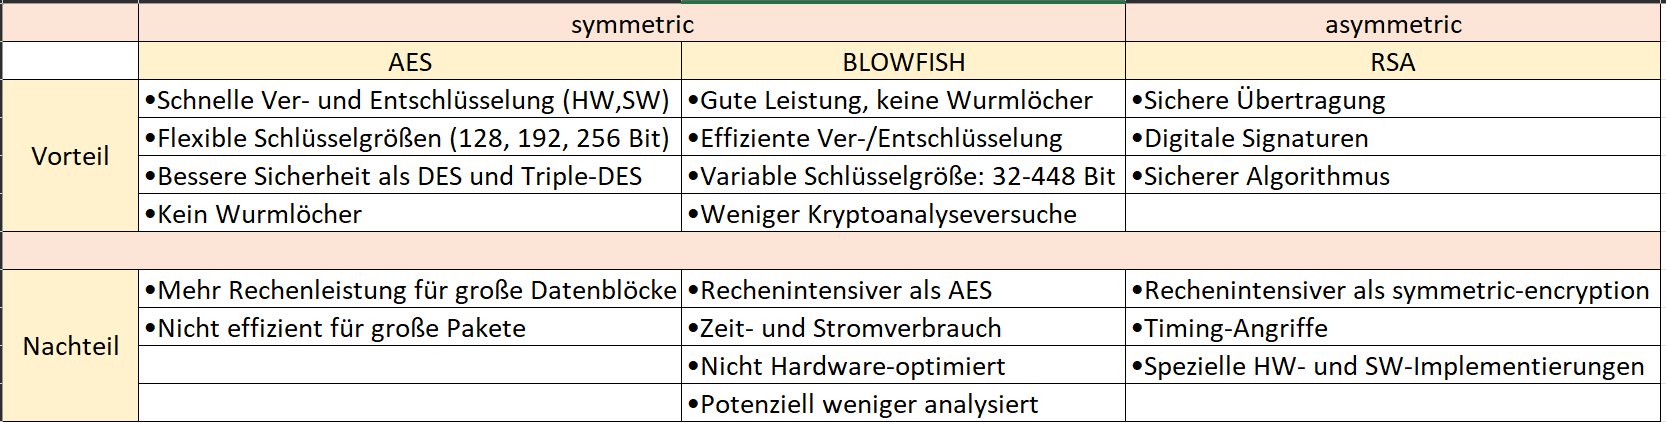
\includegraphics[scale=0.7]{resources/pic(1).png}
  \caption{}
  \label{fig:vergleich5}
\end{figure}\

\subsection{Authentifizierung}

In einer Welt, in der alles miteinander verbunden ist, ist die Authentifizierung der erste Schritt zum Schutz unserer Daten. Die Authentifizierung ist ein häufiges Sicherheitsproblem, das sich auf die Art und Weise auswirkt, wie wir Apps anzeigen, verbinden und verwenden. Für das Internet der Dinge (IoT) wurden verschiedene Authentifizierungsarten entwickelt, darunter ressourcenbeschränkte Geräte und die Cloud. Es ist wichtig zu verstehen, dass sich die Authentifizierung im Laufe der Zeit kaum verändert hat, obwohl in der heutigen technologischen Welt ein einfaches Passwort nicht mehr ausreicht, um einen Benutzer zu verifizieren.

Es gibt mehrere Authentifizierungs- und Autorisierungsmethoden für smarte Geräte. Diese Methoden beruhen auf verschiedenen Faktoren, die sich in drei Kategorien einteilen lassen \cite{khatoun2022cybersecurity}: 1. etwas, das eine Person weiß (z. B. ein Passwort oder ein Geheimcode). 
2. etwas, das eine Person ist (z. B. ein Fingerabdruck ). 
3. etwas, das eine Person besitzt (z. B. eine Chipkarte oder ein digitaler Schlüssel).
Diese Faktoren werden verwendet, um die Identität von Personen oder Systemen in Authentifizierungs- und Autorisierungsverfahren für smarte Geräte festzustellen.


Es lassen sich zwei grundlegende Arten von Authentifizierungsmechanismen unterscheiden: Intra-Domain (Authentifizierung innerhalb des Netzes) und Inter-Domain (Authentifizierung außerhalb des Netzes). Die Intra-Domain-Authentifizierung könnte durch einen der oben genannten Mechanismen erfolgen - Beweis durch Wissen, Beweis durch Besitz oder Beweis durch Eigentum. Bei der Inter-Domain-Authentifizierung sollten idealerweise zusätzliche Faktoren zum Tragen kommen, z. B. eine Kombination aus Wissens- und Besitznachweis.\cite{khatoun2022cybersecurity}


\subsubsection{Taxonomie der IoT-Authentifizierungsschemas}

Um die verschiedenen Authentifizierungsmethoden im IoT-Bereich besser zu verstehen, kann eine Taxonomie von IoT-Authentifizierungsschemas helfen.  Eine klare und strukturierte Klassifizierung bietet einen systematischen Überblick über verfügbaren Methoden und Ansätze, die zur Authentifizierung verwendet werden können. Dies erleichtert den Vergleich, die Bewertung und die Auswahl der richtigen Lösung für bestimmte Anwendungsfälle und Sicherheitsanforderungen in einer IoT-Umgebung. 
\begin{figure}[h]
  \centering
 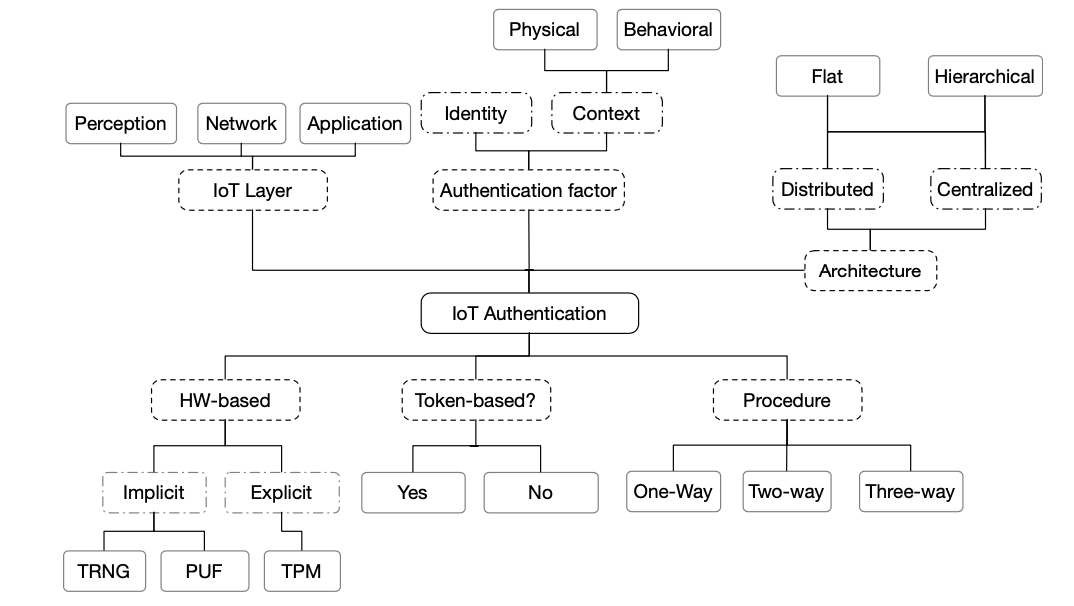
\includegraphics[scale=0.35]{resources/IoT_Auh_schems.png}
 \caption{Taxonomie der IoT-Authentifizierungsschemas \cite{el2019survey}}
  \label{fig:taxonomie}
\end{figure}\

 Hier sind einige Klassifizierungen, die in \cite{khatoun2022cybersecurity}\cite{el2019survey} erwähnt und erläutert sind:

\begin{enumerate}
        \item \textbf{Authentifizierungsfaktor:}
        \begin{enumerate}
            \item Identität: Informationen, die eine Partei der anderen zum Zwecke der Authentifizierung zur Verfügung stellt. Identitätsbasierte Authentifizierungsschemas können einen Hash-Algorithmus (oder eine Kombination davon), einen symmetrischen Verschlüsselungsalgorithmus oder einen asymmetrischen Verschlüsselungsalgorithmus verwenden. Zum Beispiel Passwortbasiert Authentifizierung.
            \item Kontext: Der Kontext kann physisch oder verhaltensbezogen sein. Ein Beispiel für einen physischen Kontext ist die biometrische Authentifizierung. 
        \end{enumerate}


    \item \textbf{Token-based:}
    \begin{enumerate}
        \item Token-basiert
        : Ein von einem Server generiertes Identitätstoken wird zur Authentifizierung verwendet, wie z. B. das OAuth2-Protokoll oder Open ID.
        \item Nicht-Token-basiert: Die Verwendung der Anmeldeinformationen(Benutzername/Passwort) bei jedem Datenaustausch.
    \end{enumerate}

    \item \textbf{Authentifizierungsarchitektur:}
    \begin{enumerate}
        \item Verteilt: Die Authentifizierung wird auf Knoten in der Nähe des Clients verteilt.
        \item Zentralisiert: Die Authentifizierung erfolgt über einen zentralen Server oder einen vertrauenswürdigen Dritten.
    \end{enumerate}

    \item \textbf{Authentifizierungsverfahren:}
    \begin{enumerate}
        \item Einweg-Authentifizierung (One-Way): Falls zwei Parteien miteinander kommunizieren möchten, wird nur eine Partei gegenüber der anderen authentifiziert und die andere Partei bleibt unauthentifiziert. Siehe Abbildung \ref{fig:one-way}.

\begin{figure}[h]
  \centering
 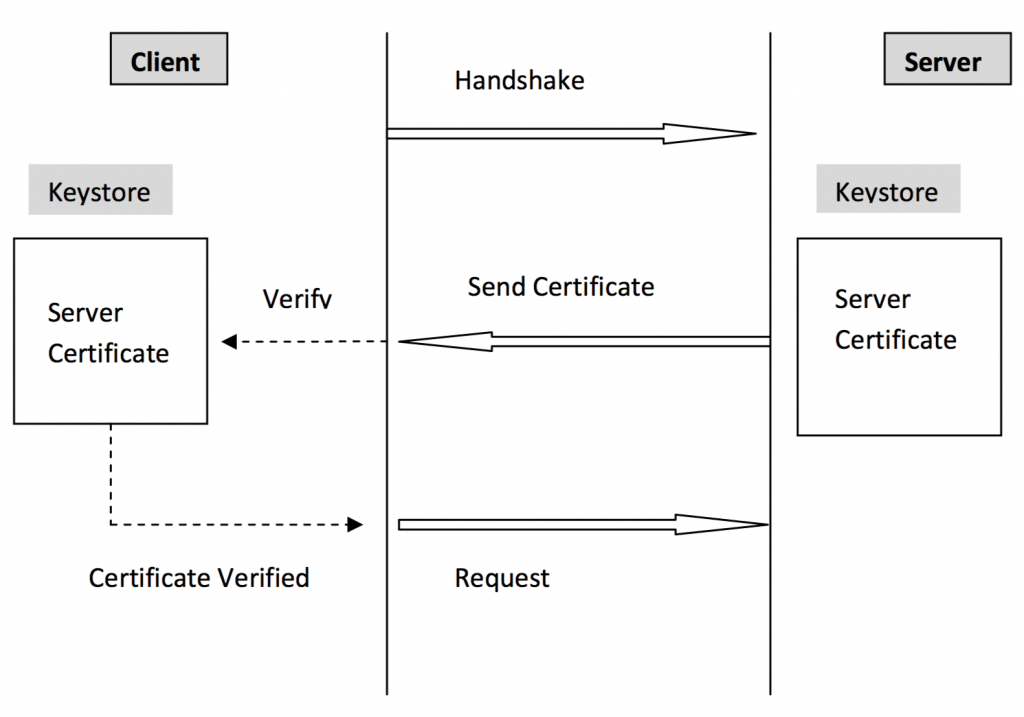
\includegraphics[scale=0.3]{resources/one-way-ssl.png}
 \caption{Einweg-Authentifizierung \href{https://raunakkathuria.github.io/blog/technical/ssl/one_way_ssl.html}{Quelle} }
  \label{fig:one-way}
\end{figure}\

 \item Zwei-Wege-Authentifizierung (Mutual): Wird auch als gegenseitige Authentifizierung bezeichnet, wenn sich beide Parteien gegenseitig authentifizieren. Dies verhindert unbefugten Zugriff und Manipulation von Gerätezuständen. 
Es gibt verschiedene Methoden der gegenseitigen Authentifizierung:
\begin{enumerate}
    \item Gegenseitige Authentifizierung unter Verwendung eines gemeinsamen Schlüssels:
 Partei A und Partei B teilen sich vorher sicher einen Schlüssel. Partei A sendet eine Nachricht an Partei B, die mit einer zufälligen Herausforderung antwortet. Partei A verschlüsselt die Herausforderung mit dem gemeinsamen Schlüssel und sendet sie Partei B zurück. Sie tauschen also verschlüsselte Herausforderungen zur Authentifizierung aus.
 \item Gegenseitige Authentifizierung mittels Public-Key-Kryptographie:
Partei A und Partei B haben jeweils ein öffentlich-privates Schlüsselpaar. Wenn A mit B kommunizieren möchte, verschlüsselt A die Nachricht mit dem öffentlichen Schlüssel von B oder signiert sie mit seinem privaten Schlüssel. B entschlüsselt die Nachricht oder verifiziert die Signatur mit seinem privaten Schlüssel.
\item Gegenseitige Authentifizierung mit Zeitstempeln:
Partei A sendet Partei B ihren aktuellen Benutzernamen und Zeitstempel mit einem gemeinsamen Schlüssel.
B entschlüsselt den Zeitstempel, erhöht ihn, verschlüsselt ihn mit einem anderen gemeinsamen Schlüssel und sendet ihn zusammen mit dem Benutzernamen an Partei A zurück. Diese Techniken geben dem Kommunikationsprozess zusätzliche Sicherheit und stellen sicher, dass beide Parteien sich gegenseitig authentifizieren, bevor sie Nachrichten austauschen.

\end{enumerate}
 

\item Drei-Wege-Authentifizierung(Three-Way): Hier authentifiziert die zentrale Autorität beide Parteien und hilft ihnen, sich gegenseitig zu authentifizieren.
  \end{enumerate}
\end{enumerate}

\subsubsection{Mutual TLS}

Gegenseitiges TLS (mTLS), auch two-way TLS genannt, ist ein Sicherheitsmechanismus, der das herkömmliche TLS-Protokoll (Transport Layer Security) erweitert. Es bietet eine gegenseitige Authentifizierung zwischen Client und Server, indem beide Parteien ihre digitalen Zertifikate zur Überprüfung bereitstellen müssen.

Bei der gegenseitigen Authentifizierung authentifizieren sich Client und Server gegenseitig mit einem digitalen Zertifikat, z.B  X.509-Zertifikatstandard, bevor sie die Kommunikation herstellen. Das X.509-Zertifikat ist der anerkannte Standard zur Authentifizierung und Zugangskontrolle in Netzwerken. Es bietet eine robuste Identitätsprüfung und sichere Kommunikation. Der weit verbreitete X.509-Zertifikatstandard umfasst einen öffentlichen Schlüssel, eine Identität, und kann von einer Zertifizierungsstelle (CA) signiert oder selbstsigniert werden.Der Prozess umfasst Root-CA-Zertifikate, Server-Zertifikate und Client-Zertifikate, die jeweils bestimmte Funktionen im Authentifizierungsprozess erfüllen \cite{khatoun2022cybersecurity} \cite{barenkamp2021iot}.

Allerdings können IoT-Geräte aufgrund ihrer begrenzten Rechenleistung Schwierigkeiten mit komplexen kryptografischen Algorithmen haben.
Um dieses Problem zu lösen, wurden neuere IoT-Geräte mit mehr Standards und erhöhter Rechenleistung entwickelt, beispielsweise das Zertifikatformat IEEE 1609.2. Diese Geräte verwenden starke kryptografische Algorithmen, die speziell für IoT-Anwendungen optimiert sind. Dadurch wird die Authentifizierung und Sicherheit in IoT-Netzwerken verbessert, ohne die Ressourcen der Geräte übermäßig zu belasten.. \cite{khatoun2022cybersecurity}

\paragraph{Die gegenseitige TLS-Authentifizierung (mTLS) funktioniert folgendermaßen:}
\

 
 Wie die Abbildung \ref{fig:mTLS} zeigt, der Client initiiert eine Verbindung zum Server. Der Server legt dem Client sein digitales Zertifikat vor, das vom Client mit Hilfe einer vertrauenswürdigen CA überprüft wird. Der Client legt dann sein eigenes Zertifikat zur gegenseitigen Authentifizierung vor, das der Server anhand einer vertrauenswürdigen CA verifiziert. Sobald beide Zertifikate erfolgreich verifiziert wurden, gewährt der Server dem Client Zugang und stellt eine sichere Verbindung für eine verschlüsselte und vertrauenswürdige Kommunikation her \cite{khatoun2022cybersecurity} \cite{barenkamp2021iot}.

  \begin{figure}[h]
  \centering
  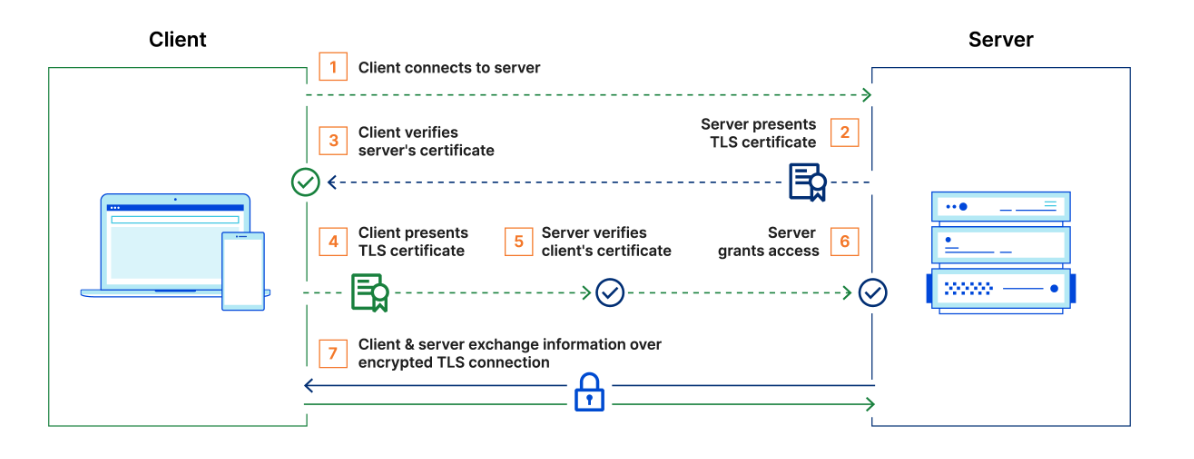
\includegraphics[scale=0.4]{resources/MUTUALTLS.png}
 \caption{TLS-Authentifizierung \href{https://www.cloudflare.com/learning/access-management/what-is-mutual-tls/}{Quelle}}
  \label{fig:mTLS}
\end{figure}\

\subsubsection{Lightweight CoAP-based Authentication }

CoAP ist eine einfachere Variante von HTTP, die für Geräte mit eingeschränkten Ressourcen entwickelt wurde. In diesem Artikel\cite{jan2014robust} wird eine vereinfachte Authentifizierungsmethode basierend auf CoAP vorgeschlagen. Dabei handelt es sich um einen einfachen Algorithmus, der eine zuverlässige Alternative zur komplexeren Data Transport Layer Security (DTLS) sein kann. Die Authentifizierung besteht aus vier Handshake-Nachrichten zwischen dem Client und dem Server unter Verwendung des 128-Bit Advanced Encryption Standard (AES). Jeder Client sendet vor Beginn der Authentifizierung einen 128-Bit-Pre-Shared-Key \(Y\textsubscript{i}\) an den Server. Jedem Gerät wird außerdem eine eindeutige Kennung zugewiesen, anhand derer der Server die Identität des Clients überprüft. Der Server verwaltet eine Pre-Shared-Key-Gruppe, die jeder Client-ID zugeordnet ist. Der Pre-Shared Key \(Y\textsubscript{i}\) ist nur dem Server und dem Client bekannt, mit dem er kommunizieren möchte. Die Authentifizierung beginnt mit der Sitzungsinitiierung. Wenn die Client-ID nicht überprüft wird, schlägt die Sitzung fehl.

Hier sind die Schritte des Authentifizierungsschemas, wie in Abbildung \ref{fig:CoAP-based-Authentication} dargestellt:

\begin{enumerate}
    \item Beginn der Sitzung:
    Der Client sendet eine Anforderungsnachricht an den Server unter Verwendung des Nachrichtentyps CON und der Methode POST. Die Nachricht enthält ein Token zur Identifizierung und eine eindeutige ID. Die Nachricht enthält auch Optionen, die die Art der Operation angeben, die an der Ressource des Servers (/authorize) durchgeführt wird. Mit dieser Anfrage wird der Server über den Beginn der Sitzung informiert.

    \item Server Challenge:
    Der Server extrahiert die Geräte-ID aus der Anfrage und findet den entsprechenden Pre-Shared Key. Es antwortet dem Client mit einer verschlüsselten Payload mithilfe des AES-Algorithmus. Der Server generiert eine Pseudozufallszahl (nonceServer) und einen potenziellen Sitzungsschlüssel \(K\textsubscript{s}\). Die verschlüsselte Payload enthält das Ergebnis der XOR-Operation zwischen \(Y\textsubscript{i}\) und \(K\textsubscript{s}\) zusammen mit dem NonceServer.
    
  AES\{Y_{i}, (Y_{i} \oplus K_{s} \mid \text{nonceServer})\}

     
    Diese Challenge muss vom Client mit \(Y\textsubscript{i}\)  entschlüsselt werden, um eine Authentifizierungssitzung aufzubauen.

    \item Client response and challenge: Der Client entschlüsselt die Challenge des Servers, um den potenziellen Sitzungsschlüssel \(K\textsubscript{s}\)  und die NonceServer zu erhalten. Ist dies erfolgreich, hat sich der Client authentifiziert. Anschließend generiert der Client eine neue verschlüsselte Payload.  Zunächst führt der Client eine XOR-Operation zwischen nonceServer und \(Y\textsubscript{i}\)  durch. Anschließend wird das Ergebnis mit nonceClient kombiniert und mit \(K\textsubscript{s}\)  verschlüsselt, wie in folgender Gleichung dargestellt  

MP = \text{AES}\{K_{s}, (nonceServer \oplus Y_{i} \mid \text{nonceClient})\}


Dabei wird die verschlüsselte Payload an den Server und die Pseudozufallszahl an den Client übertragen.

    \item Server response: Der Server prüft die verschlüsselte Payload in der Client-Antwort. Es entschlüsselt die Payload, um nonClient und nonceServer abzurufen. Wenn die Client-Antwort keinen NonceServer enthält, führt dies zu einer nicht autorisierten Serverantwort. Andernfalls wird eine neue Payload erstellt, indem der NonceClient eingefügt und \(K\textsubscript{s}\) hinzugefügt wird. Diese Payload wird mit \(Y\textsubscript{i}\) verschlüsselt.
    
M2P = AES\{\(Y\textsubscript{i}\) , (nonceClient | \(K\textsubscript{s}\))\}

 Nun sind sowohl Client als auch Server authentifiziert und können Datenpakete mit dem vereinbarten Sitzungsschlüssel \(K\textsubscript{s}\)  austauschen.

\end{enumerate}

 \begin{figure}[h]
  \centering
  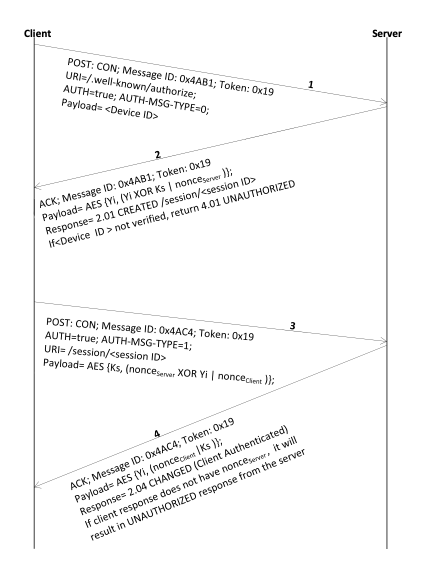
\includegraphics[scale=0.5]{resources/Lightweight CoAP-based Authentication.png}
 \caption{Lightweight CoAP-based Authentication \cite{jan2014robust}}
  \label{fig:CoAP-based-Authentication}
\end{figure}\

Das vorgeschlagene Schema ist wirksam gegen Abhören, Schlüsselgenerierung, Ressourcenerschöpfung und Denial-of-Service-Angriffe, jedoch nicht gegen Sybil-Angriffe. Es gibt jedoch keine sichere Lösung, die alle Arten von Angriffen blockieren kann \cite{jan2014robust}.


\subsubsection{CoAP Payload Based Lightweight Authentication}

In \cite{oliver2022lightweight} wird eine neue Authentifizierungsmethode zwischen CoAP-Server und CoAP-Client vorgeschlagen. Diese Methode hat mehrere Vorteile: Sie erfordert keine zusätzlichen Protokolle, was die Komplexität und den Ressourcenbedarf reduziert. Es ermöglicht die gegenseitige Authentifizierung zwischen Geräten mit nur zwei Nachrichten. Bei der Authentifizierung wird nur eine kleine Datenmenge gesendet, etwa 300 Byte. Diese Methode ist schnell und effizient, da auf beiden Geräten nur ein Roundtrip und eine Verarbeitungszeit erforderlich ist\cite{oliver2022lightweight}


Das funktioniert so: Wenn ein Client auf eine Ressource zugreifen möchte, muss er dem Server gegenüber seine Identität nachweisen. Nachdem der Server die Identität des Clients überprüft hat, erstellt er eine Sitzung für diesen Client und antwortet darauf. Nach Erhalt der Antwort authentifiziert der Client den Server. Wenn sich sowohl der Server als auch der Client gegenseitig authentifizieren, können sie mithilfe eines speziell für diese Sitzung generierten Sitzungsschlüssels Daten austauschen. Bei dieser Methode teilen sich Client und Server einen 128-Bit-AES-Schlüssel. Diese Schlüssel werden zum Zeitpunkt der Herstellung in das Gerät einprogrammiert, wobei davon ausgegangen wird, dass die Geräte vor physischen Angriffen geschützt sind. Darüber hinaus wird jedem Gerät bei der Herstellung eine eindeutige 64-Bit-ID zugewiesen.

\begin{figure}[h]
  \centering
  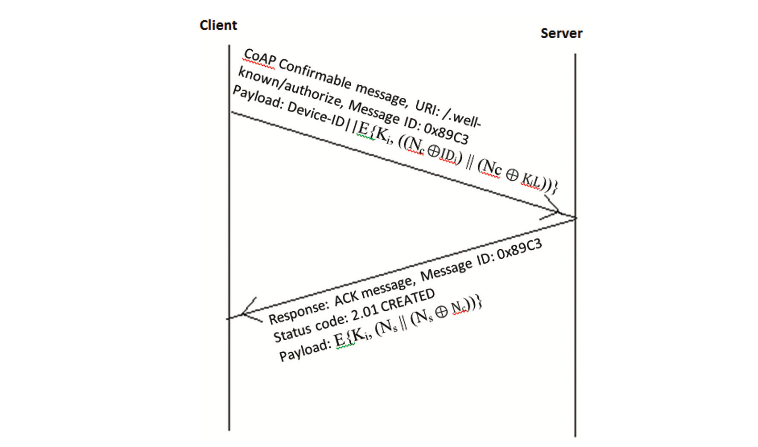
\includegraphics[scale=0.5]{resources/lightCo.png}
 \caption{CoAP Payload Based Lightweight Authentication \cite{oliver2022lightweight}}
  \label{fig:lightCo}
\end{figure}\

So funktioniert es im Detail:
Der Authentifizierungsprozess besteht aus drei Schritten: einmalige Gerätekonfiguration, Client-Authentifizierung und Server-Authentifizierung.
\begin{enumerate}
    \item \textbf{Die einmalige Gerätekonfiguration:}
Während der einmaligen Geräteeinrichtungsphase werden der eindeutige AES-Schlüssel und die eindeutige AES-ID in jedem Gerät fest codiert. Das Servergerät ist mit einer Tabelle konfiguriert, in der die Gerätekennung (\(ID\textsubscript{i}\) ) und das gemeinsame Geheimnis (\(K\textsubscript{i}\)) jedes Geräts gespeichert sind. Diese Tabelle wird verwendet, um das Gerät zu authentifizieren und den AES-Schlüssel während der ersten Servereinrichtung zu erhalten.
\item \textbf{Die Client-Authentifizierung:}
Während des Client-Authentifizierungsschritts überprüft und authentifiziert der Server die Identität des Client-Geräts. Der Client generiert eine 64-Bit-Nonce (\(N\textsubscript{c}\)) und XOR die Geräte-ID (\(ID\textsubscript{i}\) ). Nonce wird außerdem mit den niedrigstwertigen 64 Bits des gemeinsamen Clientgeheimnisses \(K\textsubscript{iL}\)  XOR-verknüpft.

\(C\textsubscript{1}\)  = E\{ {\(K\textsubscript{i}\) , ((\(N\textsubscript{c}\)  XOR  \(ID\textsubscript{i}\)) || (\(N\textsubscript{c}\) XOR \(K\textsubscript{iL}\) ))\}\

M1p = \(ID\textsubscript{i}\)  || \(C\textsubscript{1}\) 

Der Client sendet dann eine CoAP-Nachricht (\(M\textsubscript{1p}\)) an den Server.Die payload der Nachricht enthält die Geräte-ID und einen verschlüsselten Teil (\(C\textsubscript{1}\)), der mit einem gemeinsamen Geheimnis generiert wird. Die Größe der Payload-Nachricht beträgt 192 Bit, einschließlich der unverschlüsselten Gerätekennung. Der Server empfängt diese Nachricht und liest daraus die Geräte-ID. Wenn die Geräte-ID in der Tabelle gefunden wird, wird der entsprechende Pre-Shared Key abgerufen. Anschließend entschlüsselt der Server den verschlüsselten Teil (\(C\textsubscript{1}\)) mit dem gemeinsamen geheimen Schlüssel (\(K\textsubscript{i}\)), um den Klartext (\(P\textsubscript{1}\)) zu erhalten.
\(P\textsubscript{1}\) =D\{{\(K\textsubscript{i}\), (\(C\textsubscript{1}\))\}


Die höchstwertigen 64 Bits von \(P\textsubscript{1}\) werden mit der Gerätekennung IDi exklusiv-OR-verknüpft, was einen Wert \(N\textsubscript{c}\) ergibt. Die niederwertigsten 64 Bits von \(P\textsubscript{1}\) werden mit diesem \(N\textsubscript{c}\) exklusiv-OR-verknüpft, was einen Wert\(R\textsubscript{1}\) ergibt.


Der Server vergleicht den erhaltenen Wert \(R\textsubscript{1}\) mit den niederwertigsten 64 Bits des geheimen Schlüssels, der mit der Geräteidentität IDi verknüpft ist. Wenn sie übereinstimmen, wird der Client authentifiziert und eine Sitzung zwischen Client und Server aufgebaut. Stimmen die Werte nicht überein, wird eine unautorisierte Nachricht an den Client gesendet, und es wird keine Sitzung aufgebaut.

\item \textbf{Die Server-Authentifizierung:}
In der Server-Authentifizierungsphase erstellt der Server nach der Authentifizierung des Clients eine Antwortnachricht (\(M\textsubscript{2p}\)) mit dem Statuscode "2.01 created". Der Server generiert eine Nonce (\(N\textsubscript{s}\)) und führt eine exklusive OR-Operation mit der Nonce des Clients (\(N\textsubscript{c}\)) durch. 

\(M\textsubscript{2p}\) = E \{\(K\textsubscript{i}\), (\(N\textsubscript{s}\) || (\(N\textsubscript{s}\) XOR \(N\textsubscript{c}\)))\}

Die daraus resultierende Nonce \(N\textsubscript{s}\) wird dann mit der Verkettung der Nonce des Clients und der Nonce des Servers zu einem 128-Bit-Wert verkettet. Dieser Wert wird mit dem AES-Schlüssel verschlüsselt und als Payload der Antwortnachricht festgelegt.

Der Client empfängt die Antwortnachricht und entschlüsselt sie mit dem gemeinsamen geheimen Schlüssel (\(K\textsubscript{i}\)).


\(P\textsubscript{2}\) = D\{\(K\textsubscript{i}\), \(M\textsubscript{2p}\)\}

Die entschlüsselte Payload (\(M\textsubscript{2p}\)) wird dann verarbeitet, und die niedrigstwertigen 64 Bits des Klartextes (\(P\textsubscript{2}\)) werden mit den höchstwertigen 64 Bits von \(P\textsubscript{2}\) exklusiv-OR-verknüpft, was zu einem Wert \(R\textsubscript{2}\) führt.

Der Client vergleicht den Wert \(R\textsubscript{2}\) mit seiner eigenen Nonce (\(N\textsubscript{c}\)), um den Server zu authentifizieren. Wenn sie übereinstimmen, ist der Server authentifiziert, was bedeutet, dass nur der beabsichtigte Server die Nachricht des Clients entschlüsselt und die verschlüsselte Nonce zurückgeschickt haben kann.
\end{enumerate}


Sobald die gegenseitige Authentifizierung zwischen Client und Server erreicht ist, wird ein Sitzungsschlüssel (\(K\textsubscript{s}\)) durch Verkettung der Nonce des Clients (\(N\textsubscript{c}\)) mit der Nonce des Servers (\(N\textsubscript{s}\)) erzeugt. Dieser Sitzungsschlüssel wird zum Ver- und Entschlüsseln der während der authentifizierten Sitzung übertragenen Daten verwendet. Der während der Herstellungsphase gemeinsam genutzte AES-Schlüssel wird ausschließlich zu Authentifizierungszwecken verwendet, was die Sicherheit des Systems erhöht.

\subsection{Zugriffskontrolle und Berechtigungen}

Die Integration der physischen Welt und des Cybersystems im Internet der Dinge stellt große Herausforderungen an die Gestaltung von Sicherheitslösungen. Die Zugangskontrolle gilt als kritische Systemkomponente zum Schutz von Daten und Cyber-Infrastruktur. Aufgrund der neuen Eigenschaften von IoT-Systemen, wie z. B. viele traditionelle Sicherheitslösungen, einschließlich vorhandener Zugriffskontrollmechanismen, sind jedoch möglicherweise nicht direkt in der IoT-Umgebung anwendbar, z. B. Ressourcenbeschränkung, großer Umfang und Geräteheterogenität.\cite{8038503}\cite{ouaddah2017access}

\subsubsection{Zugriffskontrollmechanismen}

Ein vollständiges Zugangskontrollsystem besteht aus drei Funktionen: Authentifizierung, Autorisierung und Verantwortlichkeit. Der Zugriffskontrollmechanismus, der Hardware und Software umfasst, setzt Richtlinien durch und wertet Zugriffsanfragen aus. Die Konfiguration der Zugriffskontrollrichtlinien ist von entscheidender Bedeutung und sollte regelmäßig überprüft und verifiziert werden. Tools wie ACLs, Router, Verschlüsselung, Prüfprotokolle, IDS, Antivirensoftware, Firewalls, Smartcards und Warnungen sind Teil dieses Systems\cite{ouaddah2017access},\cite{vollbrecht2000rfc2904},\cite{boyle2007survey},\cite{hu2011anomaly},\cite{ledru2011validation}.
Es gibt viele verschiedene Zugriffskontrollmechanismen wie Role-Based Access Control (RBAC), Attribute-Based Access Control (ABAC) , Mandatory Access Control (MAC), Discretionary Access Control (DAC), Multi-Factor Authentication (MFA) und Single Sign-On (SSO) und Secure Shell (SSH), aber wir konzentrieren uns nur auf RBAC und ABAC\cite{ouaddah2017access}, \cite{coyne2013abac}, \cite{ameer2022hybrid}\cite{ali2019internet}\cite{dutta2020context}.

\subsubsection{RBAC und ABAC}

Obwohl ABAC und RBAC ähnlich sind, haben sie Vor- und Nachteile. Bei kluger Kombination kann die Kombination eine skalierbare, flexible, überprüfbare und verständliche Zugangskontrolle bieten. Durch die Kombination von Rollenzentrierung, dynamischen Rollenfunktionen und der feinkörnigen Autorisierung von ABAC demonstriert es die Praktikabilität des in ANSI/INCITS 494-2012 definierten Ansatzes und bietet eine Kombination der besten Funktionen von RBAC und ABAC für Unternehmen.
RBAC ist weit verbreitet und bietet Verwaltungs- und Sicherheitsvorteile. Es ist jedoch veraltet, teuer in der Implementierung und nicht in der Lage, Echtzeit-Umgebungszustände als Zugangskontrollparameter zu berücksichtigen. ABAC hingegen ist neuer, einfacher zu implementieren und kann Echtzeit-Umgebungszustände als Zugangskontrollparameter berücksichtigen.

Einerseits basiert die Zugriffskontrolle in RBAC auf vordefinierten Rollen und Berechtigungen, und Benutzerzugriffsentscheidungen hängen in erster Linie von den ihnen zugewiesenen Rollen ab. RBAC vereinfacht die Verwaltung, indem es die Zugriffskontrolle nach Rollen organisiert. Andererseits basiert die Zugriffskontrolle in ABAC auf verschiedenen Merkmalen von Benutzern, Objekten und der Umgebung, und Zugriffsentscheidungen berücksichtigen Attribute wie Benutzerrolle, Abteilung, Standort usw. ABAC bietet eine feinkörnige und kontextbezogene Steuerung von Genehmigung.

Sowohl RBAC als auch ABAC können verwendet werden, indem Rollen als Benutzerattribute betrachtet werden. RBAC vereinfacht die Administration und eignet sich für Organisationen mit komplexen Benutzerstrukturen. ABAC bietet Flexibilität, Granularität und feinkörnige Zugriffskontrolle. Darüber hinaus können Attribute zu RBAC hinzugefügt werden, um die erforderliche Flexibilität bei der Zugriffskontrolle zu erreichen.

RBAC ist einfacher zu implementieren, während ABAC eine Eigenschafts- und Richtlinienverwaltung erfordert. ABAC eignet sich besonders für dynamische Umgebungen und Attribute wie Tageszeit und Standort und ermöglicht eine effektive Richtliniendurchsetzung\cite{coyne2013abac}\cite{ameer2022hybrid}.

\begin{figure}[h]
  \centering
  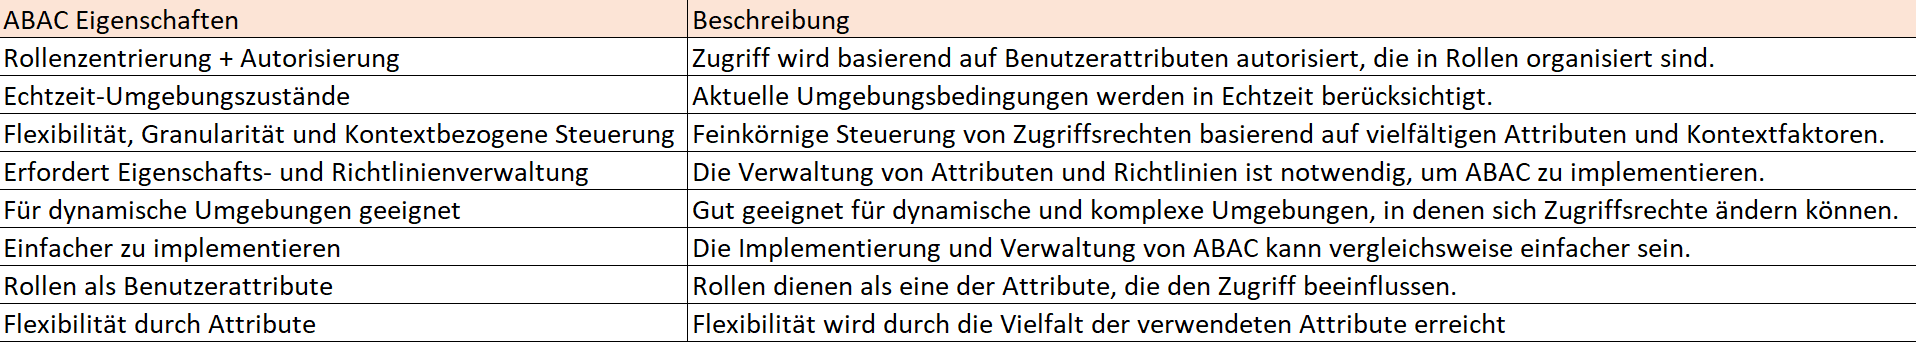
\includegraphics[scale=0.64]{resources/pic(2).png}
  \caption{}
  \label{fig:vergleich6}
\end{figure}\

\begin{figure}[h]
  \centering
  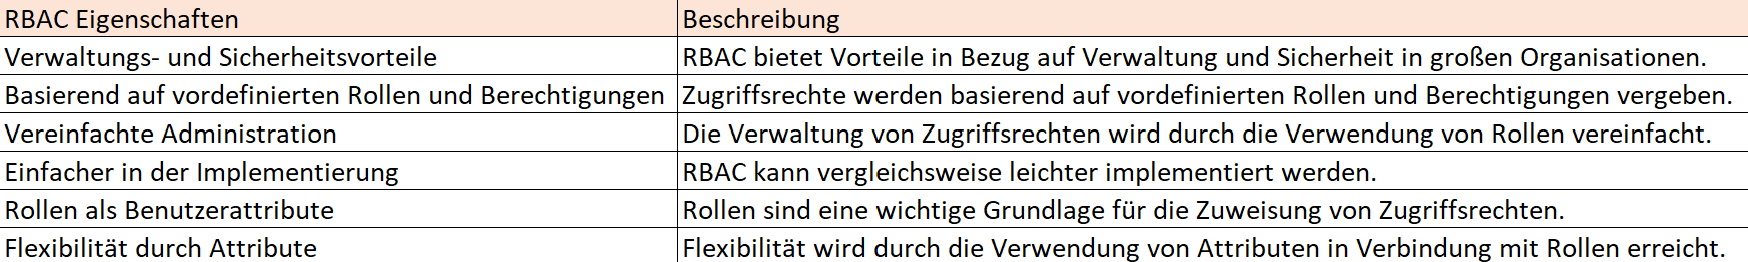
\includegraphics[scale=0.7]{resources/pic(3).png}
  \caption{}
  \label{fig:vergleich7}
\end{figure}\


\subsubsection{HyBACAC}
Durch die vorteilhafte Kombination zweier Modelle, ABAC und R, als Hybridansatz steht eine umfassendere und wandelbarere Zutrittskontrolllösung zur Verfügung.
Ein von RBAC bereitgestelltes rollenzentriertes Framework vereinfacht die Administration und Zugriffsverwaltung, indem Berechtigungen an Rollen statt an einzelne Benutzer vergeben werden. Dies verbesserten die Skalierbarkeit und Ausdauer.
Andererseits kann ABAC eine feinkörnige Zugriffskontrolle unter Berücksichtigung der Attribute von Benutzern, Geräten und der Umgebung durchführen, was eine dynamische Entscheidungsfindung auf der Grundlage verschiedener Kontextfaktoren ermöglicht.
HyBACAC kann von der rollenbasierten Einfachheit von RBAC und der attributbasierten Flexibilität von ABAC profitieren. Diese Kombination erleichtert Administratoren das Definieren von Rollen und das Zuweisen geeigneter Berechtigungen, indem dynamische Attribute berücksichtigt werden, um den Zugriff weiter einzuschränken.
Es ermöglicht das Prinzip der geringsten Rechte und eine einfache Überprüfung der Benutzerberechtigungen.
Das Hybridmodell ist in der Lage, plötzliche Attributänderungen und Kontextinformationen durch dynamische Attribute und Umgebungsrollen zu erfassen. Dadurch wird sichergestellt, dass Entscheidungen zur Zugangskontrolle, an die sich ändernden Bedingungen in intelligenten IoT-Systemen angepasst werden können\cite{ameer2022hybrid}.

\begin{figure}[h]
  \centering
 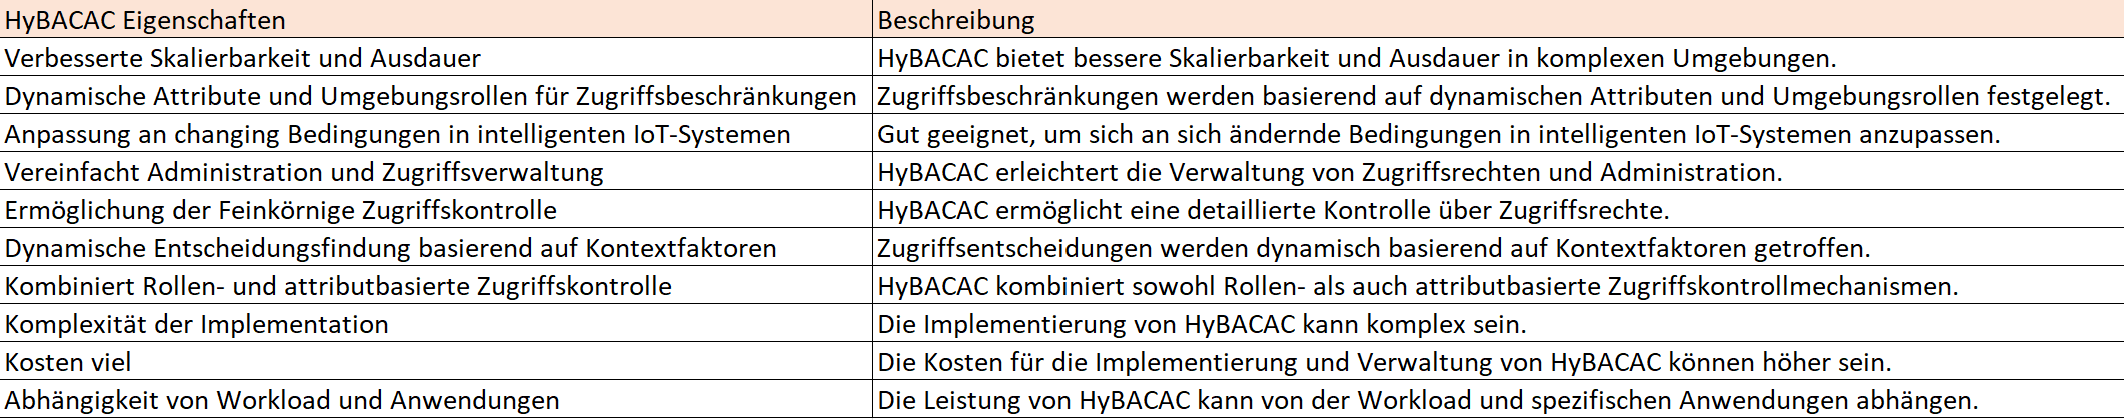
\includegraphics[scale=0.6]{resources/pic(4).png}
  \caption{}
  \label{fig:vergleich7}
\end{figure}\


\section{Zusammenfassung}

In diesem Artikel haben wir uns mit den  grundlegenden Konzepten des Internet der Dinge (IoT) befasst, insbesondere im Zusammenhang mit Smart-Home Netzwerken.  Dabei wurden  Risiken und Bedrohungen beleuchtet, wie zum Beispiel absichtliche Cyberangriffe, unbeabsichtigte Fehler und Fehlfunktionen sowie Malware-Infektionen und Denial-of-Service-Angriffe. Um diese Netzwerke zu schützen, sind entsprechende  Schutzmechanismen von großer Bedeutung und müssen deswegen eingesetzt werden. Verschiedene Verschlüsselungstechnologien wie AES, RSA und BLOWFISH wurden diskutiert, wobei sich AES als effizienter und sicherer als andere erwiesen hat.Zudem haben wir eine Reihe nützlicher Authentifizierungsmethoden wie Mutual TLS, Lightweight CoAP-based Authentication und CoAP Payload Based Lightweight Authentication vorgestellt.  Lightweight CoAP-based Authentication und CoAP Payload Based Authentication sind ideal für eingeschränkte Geräte. CoAP Payload Based Lightweight Authentication ist jedoch etwas schneller und erfordert nur zwei Handshakes für eine vollständige Authentifizierung. Außerdem ist eine effektive Zugangskontrolle durch ABAC, RBAC und insbesondere HybACAC erforderlich, um unbefugten Zugriff zu verhindern.  

Keywords: 
Smart Home Netzwerke, Architektur, Kommunikationsprotokolle, Bedrohungen, Risiken, Schutzmechanismen, Sicherheit, Verschlüsselung, Authentifizierung, Zugriffskontrolle, AES, BLOWFISH, RSA, Mutual TLS, Lightweight CoAP-based Authentication, CoAP Payload Based Lightweight Authentication, Zugriffskontrollmechanismen, IoT, Netzwerksicherheit, Datenschutz, Netzwerkarchitektur, Schwachstellen, Sicherheitslücken, Netzwerkprotokolle, Cybersecurity, Sichere Kommunikation, Risikomanagement.


\newpage
\paragraph{Was? Wer?}\

\textbf{Architektur von Smart Home-Netzwerken:} Aiman

\textbf{Kommunikationsprotokolle in Smart Home-Netzwerken:} Aiman

\textbf{Bedrohungen und Risiken für Smart Home-Netzwerke:} Zohreh

\textbf{Wichtige Schutzmechanismen zur Sicherung von Smart Home-Netzwerken:} Aiman

\textbf{Verschlüsselungstechnologien:} Zohreh

\textbf{Authentifizierung:} Aiman

\textbf{Zugriffskontrolle und Berechtigungen:} Zohreh

\newpage
    \nocite{*}
    \bibliography{src/referencias}


\end{document}
